%%%%%%%%%%%%%%%%%%%%%%%%%%%%%%%%%%%%%%%%%%%%%%%%%%%%%%%%%%%%%%%%%%%%%%%%%%%%%%%
%  Trabajo final de Arquitectura de Computadoras (I-60)
%  RISC-V RV32I segmentado de 5 etapas con Debug Unit por UART, en una Basys 3
%
%  Estructura:
%     main.tex                carátula, preámbulo y orden de las secciones
%     informe-fcefyn.sty      plantilla de informes de la FCEFyN
%     secciones/*.tex         una sección por archivo
%     img/                    logos
%  Las figuras se toman de ../diagramas, ../capturas y ../timing sin copiarlas
%  (\graphicspath): el informe usa los mismos PNG que el resto de docs/.
%
%  Compilar desde la raíz del repo (la salida va a build/, que no se versiona):
%     latexmk -pdf -outdir=build/informe -cd docs/informe/main.tex
%  En Overleaf: subir la carpeta docs/ entera y elegir informe/main.tex como
%  documento principal (ver docs/informe/README.md).
%
%  Lo que aparece entre corchetes rojos (\completar{...}) falta llenarlo.
%  Para la entrega, descomentar \entregafinal.
%%%%%%%%%%%%%%%%%%%%%%%%%%%%%%%%%%%%%%%%%%%%%%%%%%%%%%%%%%%%%%%%%%%%%%%%%%%%%%%
\documentclass[11pt,a4paper]{article}
% Compilando desde docs/ (Overleaf con informe/main.tex como documento principal)
% los archivos del informe se buscan también en informe/.
\makeatletter
\IfFileExists{secciones/01_introduccion.tex}{}{\def\input@path{{informe/}}}
\makeatother
\usepackage{informe-fcefyn}

\entregafinal

% ------------------------- Datos de la carátula ------------------------------
\materia{Arquitectura de Computadoras}
\carrera{Ingeniería en Computación}
\subtitulo{Trabajo Final}
\tema{Procesador RISC-V segmentado con Debug Unit}
\plataforma{Basys 3 (Artix-7 \texttt{xc7a35tcpg236-1}) \textperiodcentered{} Verilog \textperiodcentered{} Vivado 2024.2 \textperiodcentered{} Python}
\autor{Costamagna, Matías}{44.512.437}{matias.costamagna@mi.unc.edu.ar}
\autor{Moreyra, Julián}{45.214.537}{julian.moreyra@mi.unc.edu.ar}
\docentes{Martín Alonso, Martín Pereyra}
\fechaentrega{27 de noviembre de 2026}
\logoizquierdo{img/unc_logo.png}
\logoderecho{img/fcefyn_logo.jpg}

% Las figuras salen de las carpetas de docs/. Las dos variantes de cada ruta
% cubren compilar con -cd (desde docs/informe) y compilar desde docs/ (Overleaf
% con la carpeta docs/ como proyecto).
\graphicspath{{img/}{../diagramas/}{../capturas/}{../timing/}%
              {informe/}{informe/img/}{diagramas/}{capturas/}{timing/}}

\newcommand{\Repo}{https://github.com/moreyrajulian/arquitectura_de_computadoras}

% ---------------------------- Estilo de Verilog -------------------------------
% La plantilla trae el estilo de C (cmcx); el RTL del trabajo es Verilog.
\lstdefinestyle{verilog}{
  style=cmcx, language=Verilog,
  morekeywords=[2]{wire,reg,input,output,localparam,parameter},
}

% Figura con un diagrama de docs/diagramas a todo el ancho
% \diagrama[ancho]{archivo}{título}{descripción}{etiqueta}
\newcommand{\diagrama}[5][\linewidth]{%
  \begin{figure}[H]
    \centering
    \IfFileExists{../diagramas/#2}{\includegraphics[width=#1,height=0.72\textheight,keepaspectratio]{#2}}{%
      \IfFileExists{diagramas/#2}{\includegraphics[width=#1,height=0.72\textheight,keepaspectratio]{#2}}{%
        \completar{Falta \texttt{docs/diagramas/\detokenize{#2}}}}}
    \caption{\textbf{#3.} #4}
    \label{#5}
  \end{figure}}

% \captura de la plantilla busca el archivo solo en la carpeta actual (no usa
% \graphicspath) y las capturas están en docs/capturas: se redefine igual que
% \diagrama, con un recuadro rojo si el archivo no existe.
% \captura[alto]{archivo}{título}{descripción}{etiqueta}
\renewcommand{\captura}[5][0.42\textheight]{%
  \begin{figure}[H]
    \centering
    \IfFileExists{../capturas/#2}{\includegraphics[width=0.95\linewidth,height=#1,keepaspectratio]{#2}}{%
      \IfFileExists{capturas/#2}{\includegraphics[width=0.95\linewidth,height=#1,keepaspectratio]{#2}}{%
        \completar{Falta \texttt{docs/capturas/\detokenize{#2}}}}}
    \caption{\textbf{#3.} #4}
    \label{#5}
  \end{figure}}

% Referencia a un archivo del repositorio
% Rutas y nombres largos: se pueden cortar en / _ . -
\makeatletter\g@addto@macro\UrlBreaks{\do\_\do\-}\makeatother
\newcommand{\repo}[1]{\nolinkurl{#1}}
% Decisión de diseño: \decision{012}
\newcommand{\decision}[1]{decisión~#1}

\begin{document}

\caratula
\setcounter{tocdepth}{2}
\tableofcontents
\newpage

% ===========================================================================
\section{Introducción}
\label{sec:intro}

\begin{consigna}[Trabajo final \textemdash{} Pipeline del procesador RISC-V]
\small\raggedright\setlength{\parskip}{4pt}
\textbf{Consigna.} Implementar el pipeline del procesador RISC-V (etapas IF, ID, EX, MEM y WB);
una Debug Unit que permita enviar y recibir información al procesador mediante protocolo UART, y
una interfaz para visualizar los datos e interactuar con la Debug Unit (CLI, GUI y/o TUI).

\textbf{Instrucciones a implementar.}
\begin{itemize}[nosep]
  \item R-type: \texttt{add, sub, sll, srl, sra, and, or, xor, slt, sltu}.
  \item I-type: \texttt{lb, lh, lw, lbu, lhu, addi, andi, ori, xori, slti, sltiu, slli, srli,
        srai, jalr}.
  \item S-type: \texttt{sb, sh, sw}. \quad B-type: \texttt{beq, bne}. \quad J-type:
        \texttt{jal}. \quad U-type: \texttt{lui}.
\end{itemize}

\textbf{Requerimientos.} El procesador debe poder programarse y reprogramarse con comandos por
UART, sin resintetizar. El clock no debe verse intervenido en ninguna parte del proyecto. Las
decisiones de diseño se documentan con su porqué.

\textbf{Debug Unit.} Se envían a la PC por la UART el contenido de los 32 registros, de los
latches intermedios y de la memoria de datos usada.

\textbf{Carga de programa.} El programa está escrito en ensamblador, con un mecanismo para
traducirlo a lenguaje máquina y una instrucción HALT. El sistema permite programar el procesador
escribiendo la memoria de programa, reprogramarlo de manera dinámica, y responde: ¿es necesario
vaciar la memoria?, ¿y los registros?, ¿se necesita vaciar el pipeline?, ¿y la memoria de
programa?

\textbf{Modos de operación.} Continuo (un comando ejecuta el programa hasta el final y se
muestran todos los valores) y paso a paso (cada comando ejecuta un ciclo de clock y se muestran
los valores). En ambos casos el pipeline debe quedar vacío al terminar. Responder: ¿qué sucede si
en la memoria no se encuentra una instrucción de parada?

\textbf{Clock.} En la integración: ¿cuál es el camino crítico del sistema?, ¿genera skew y qué
consecuencias tiene? De encontrarse skew, encontrar la frecuencia óptima, generar métricas con
las herramientas de Vivado y aplicar esa frecuencia.
\end{consigna}

El trabajo final de la materia es un procesador \textbf{RISC-V RV32I segmentado en cinco etapas}
(IF, ID, EX, MEM, WB), con unidad de cortocircuitos (\emph{forwarding}), detección de riesgos y
una \textbf{Debug Unit} que se comunica con la PC por UART. Está escrito en Verilog, se implementa
en una Basys~3 (Artix-7 \texttt{xc7a35tcpg236-1}) con Vivado~2024.2 y se maneja desde la PC con un
debugger de texto propio.

Desde la PC se puede cargar un programa en ensamblador sin volver a sintetizar, ejecutarlo de
corrido o de a un ciclo por comando, y ver en cada paso los 32 registros, los cuatro registros de
segmentación, la memoria de datos usada y qué instrucción hay en cada etapa.

\subsection{Resultados}

\begin{itemize}[nosep]
  \item \textbf{ISA}: el subset RV32I de la consigna (32 instrucciones) más \texttt{halt}
        (\texttt{ebreak}), sección~\ref{sec:isa}.
  \item \textbf{Pipeline}: cinco etapas con forwarding desde EX/MEM y MEM/WB, bypass en el banco
        de registros, un ciclo de \emph{stall} por carga-uso y saltos resueltos en EX con
        \emph{flush} de dos ciclos (secciones~\ref{sec:pipeline} y~\ref{sec:riesgos}).
  \item \textbf{Debug Unit}: protocolo de tramas con checksum, 14 comandos y dos máquinas de
        estado, sin tocar el reloj: el core avanza o se detiene con una señal
        \texttt{enable} (sección~\ref{sec:debug}).
  \item \textbf{Reloj}: \qty{92}{\mega\hertz} con el Clock Wizard, la máxima frecuencia de un
        barrido de 65 a \qty{100}{\mega\hertz} que cumple timing (slack $+0{,}026$~ns,
        sección~\ref{sec:timing}).
  \item \textbf{Verificación}: dos oráculos independientes (estado final escrito a mano y un
        modelo de referencia ciclo a ciclo), un banco que compara los cuatro registros de
        segmentación en cada ciclo, 39 mutantes del RTL y la prueba en la placa: 22 de 22
        programas con ejecución continua y paso a paso, y 32 de 32 de las variantes sin
        riesgos (sección~\ref{sec:verif}).
  \item \textbf{Herramientas}: ensamblador, modelo de referencia, debugger con interfaz de texto y
        scripts de regresión, timing y prueba en placa (secciones~\ref{sec:interfaz}
        y~\ref{sec:uso}).
\end{itemize}

\subsection{Repositorio}
\label{sec:repo}

\begin{nota}[Código, documentación y evidencia]
\centering\normalsize
\url{\Repo}\par\smallskip
\small Versión descripta en este informe: tag \href{\Repo/tree/v1.0}{\texttt{v1.0}}
\end{nota}

Este informe resume el trabajo; lo completo está en el repositorio: el RTL, los testbenches, los
programas de prueba, las herramientas de la PC, la especificación, las 45 notas de decisión y los
reportes de Vivado. Las rutas que aparecen en el texto con este formato, como
\repo{docs/spec/pipeline.md} o \repo{tools/debugger/}, son relativas a la raíz del repositorio.
Para empezar conviene leer:

\begin{itemize}[nosep]
  \item \href{\Repo\#readme}{\texttt{README.md}}: estado, estructura y cómo usar el procesador.
  \item \href{\Repo/tree/master/docs}{\texttt{docs/}}: especificación, decisiones, diagramas,
        timing y capturas de la placa.
  \item \href{\Repo/tree/master/sw/demo}{\texttt{sw/demo/}}: los programas de demostración y el
        guion para recorrerlos con el debugger.
  \item \href{\Repo/blob/master/docs/informe/presentacion.pdf}{\texttt{docs/informe/presentacion.pdf}}:
        la presentación del trabajo.
\end{itemize}

\subsection{Cómo está organizado el trabajo}

Este informe resume y enlaza la documentación del repositorio:

\begin{center}
\small
\begin{tabular}{@{}p{4.2cm} p{11.4cm}@{}}
  \toprule
  \textbf{Carpeta} & \textbf{Contenido} \\
  \midrule
  \repo{docs/spec/}        & Especificación escrita antes del código: ISA, pipeline, memorias, protocolo, interfaz y verificación \\
  \repo{docs/decisiones/}  & 45 notas de decisión de diseño, con las opciones y el porqué (anexo~\ref{anx:decisiones}) \\
  \repo{docs/timing/}      & Reportes de Vivado, camino crítico, skew y barrido de frecuencias \\
  \repo{rtl/}, \repo{fpga/}, \repo{ip/} & Diseño sintetizable, top de la placa y scripts de los IP cores \\
  \repo{tb/}               & Testbenches unitarios y el banco de pruebas del pipeline \\
  \repo{sw/}               & Programas de prueba en ensamblador con su resultado esperado \\
  \repo{tools/}            & Ensamblador, modelo de referencia y debugger \\
  \repo{scripts/}          & Proyecto de Vivado, regresión, timing y barrido \\
  \bottomrule
\end{tabular}
\end{center}

\paragraph{Metodología.} El pipeline se construyó \textbf{etapa por etapa}: cada etapa fue un
hito con sus módulos, sus testbenches unitarios y una integración verificada contra el modelo de
referencia antes de pasar a la siguiente. Los riesgos se agregaron recién con las cinco etapas
funcionando, porque involucran a varias a la vez. Cada tarea fue una issue de GitHub (se citan
como I-NN) con sus criterios de terminado, una rama y un pull request revisado por el otro
integrante. Antes de escribir un módulo se documentó su interfaz en \repo{docs/spec/}, y cada
decisión de diseño quedó en una nota numerada. La planificación por hitos está en
\repo{docs/planificacion.md}; el avance real, en las issues y los pull requests del repositorio.

% ===========================================================================
\section{Arquitectura del sistema}
\label{sec:sistema}

\diagrama{sistema.png}{Vista de sistema}{Bloques, interfaces y quién controla a quién. La PC
nunca accede directamente al core ni a las memorias: todo entra por la UART y lo interpreta la
Debug Unit. Fuente editable: \repo{docs/diagramas/sistema.drawio}.}{fig:sistema}

El diseño de la placa (\repo{fpga/riscv_basys3/top.v}) tiene cinco bloques
(figura~\ref{fig:sistema}):

\begin{description}[style=nextline,nosep,leftmargin=1.2em]
  \item[Clock Wizard (MMCM)] Genera desde los \qty{100}{\mega\hertz} de la placa el único reloj
        del sistema, \qty{92}{\mega\hertz} (\decision{045}). Hasta que el MMCM engancha
        (\texttt{locked}) todo queda en reset.
  \item[Reset] El botón central, sincronizado y alargado por \repo{rtl/common/reset_sync.v},
        más el reset de encendido (\decision{041}).
  \item[UART] La del TP2 (receptor, transmisor y generador de baudios con sobremuestreo
        $16\times$) con una FIFO de recepción, a 115200~baudios 8N1 (decisiones 003 y 035).
  \item[Debug Unit] Interpreta las tramas de la PC, carga el programa por el puerto~B de la
        memoria de programa, genera \texttt{enable} y \texttt{core\_rst} y vuelca el estado del
        core (sección~\ref{sec:debug}).
  \item[Core] El procesador segmentado con sus dos memorias BRAM: la de programa (IF) y la de
        datos (MEM), de 1024 palabras cada una (secciones~\ref{sec:pipeline}
        a~\ref{sec:memorias}).
\end{description}

\subsection{Un solo dominio de reloj}

La consigna prohíbe intervenir el reloj. El diseño tiene \textbf{un único reloj}, que sale del
MMCM por un BUFG y llega a todos los elementos sincrónicos: core, memorias, Debug Unit y UART. No
hay \emph{clock gating}, divisores ni relojes generados con lógica.

Parar o avanzar el core se hace con una señal \texttt{enable} que maneja la Debug Unit: todo
elemento con estado del core (PC, registros de segmentación, escritura del banco y de la memoria
de datos, registro \texttt{halted} y avisos) solo se actualiza en los flancos con
\texttt{enable = 1} (\decision{018}). En la serie 7 cada flip-flop tiene su entrada de
\emph{clock enable} (CE), así que esto no agrega lógica en el camino de datos: usa el CE. Un
\texttt{STEP} es \texttt{enable = 1} durante un ciclo de reloj; mientras tanto el reloj sigue
corriendo para la UART y la Debug Unit, que pueden leer el estado del core detenido por puertos
propios (el puerto~B de las BRAM y un tercer puerto de lectura del banco).

La sección~\ref{sec:skew} muestra la consecuencia medida: el skew del reloj es de decenas de
picosegundos, menor que el jitter del MMCM.

\subsection{LEDs de la placa}

Para saber si la FPGA responde aunque no responda la UART, el top muestra el estado en los LEDs:

\begin{center}
\small
\begin{tabular}{@{}l l@{}}
  \toprule
  \textbf{LED} & \textbf{Significado} \\
  \midrule
  LD0 a LD4   & Estado de ejecución, uno encendido: \texttt{NO\_PROG}, \texttt{READY}, \texttt{RUNNING}, \texttt{PAUSED}, \texttt{HALTED} \\
  LD8 a LD10  & Avisos de acceso: \texttt{imem\_fault}, \texttt{dmem\_oob}, \texttt{dmem\_misaligned} \\
  LD14        & Reset del sistema activo \\
  LD15        & Latido de \qty{2}{\hertz}; quieto significa sin reloj o con el reset apretado \\
  \bottomrule
\end{tabular}
\end{center}

% ===========================================================================
\section{Conjunto de instrucciones}
\label{sec:isa}

El procesador implementa el subset de RV32I que pide la consigna más una instrucción de parada
(\repo{docs/spec/isa.md}):

\begin{center}
\small
\begin{tabular}{@{}l l l@{}}
  \toprule
  \textbf{Tipo} & \textbf{Formato} & \textbf{Instrucciones} \\
  \midrule
  Aritméticas y lógicas    & R & \texttt{add sub sll srl sra and or xor slt sltu} \\
  Con inmediato            & I & \texttt{addi andi ori xori slti sltiu slli srli srai} \\
  Cargas                   & I & \texttt{lb lh lw lbu lhu} \\
  Almacenamientos          & S & \texttt{sb sh sw} \\
  Saltos condicionales     & B & \texttt{beq bne} \\
  Saltos incondicionales   & J, I & \texttt{jal jalr} \\
  Inmediato superior       & U & \texttt{lui} \\
  Parada                   & I & \texttt{halt} (= \texttt{ebreak}, \texttt{0x00100073}) \\
  \bottomrule
\end{tabular}
\end{center}

\diagrama{formatos.png}{Formatos de instrucción}{Los seis formatos de RISC-V y, para cada uno con
inmediato, de qué bits de la instrucción sale cada bit del inmediato de 32 bits. Los colores
identifican el bit de origen y son los mismos en todos los formatos.}{fig:formatos}

\subsection{La instrucción de parada}
\label{sec:halt}

La consigna pide una instrucción que detenga el procesador con el pipeline vacío. Se codificó como
\texttt{ebreak} (\texttt{0x00100073}) porque no choca con ninguna instrucción implementada, el
ensamblador estándar la genera y no exige herramientas propias (\decision{001}).

Viaja por el pipeline como una instrucción sin efectos que solo lleva su bit \texttt{halt}.
Mientras haya un HALT en cualquier etapa, IF deja de buscar:

\begin{lstlisting}[style=verilog,numbers=none]
stop_fetch  = id_is_halt | id_ex_halt | ex_mem_halt | mem_wb_halt | halted;
flush_if_id = redirect | stop_fetch;
\end{lstlisting}

\texttt{stop\_fetch} congela el PC y además convierte en burbuja lo que entra a IF/ID. Hacen falta
las dos cosas: cuando el HALT está en ID, la BRAM ya está leyendo la dirección siguiente y esa
palabra aparecería en IF/ID en el flanco siguiente. La parada mira las cuatro etapas porque el HALT
está en ID un solo ciclo. Cuando llega a WB se levanta \texttt{halted} y el pipeline queda vacío
(los cuatro \texttt{valid} en 0).

Hay dos casos borde que la verificación cubre con programas propios:
\begin{itemize}[nosep]
  \item \textbf{HALT en el camino equivocado}: si un salto anterior se toma, el \emph{flush}
        convierte al HALT en burbuja, su bit desaparece y \texttt{stop\_fetch} se apaga solo
        (\repo{sw/halt_camino_equivocado.s}).
  \item \textbf{HALT retenido por un stall}: \texttt{0x00100073} tiene un 1 en el campo
        \texttt{rs2}, así que un \texttt{lw x1} justo antes dispara la detección de carga-uso.
        Como el \emph{enable} tiene prioridad sobre el \emph{flush}, IF/ID conserva el HALT
        (\repo{sw/halt_stall.s}).
\end{itemize}

\subsection{Instrucciones fuera del subset}

La unidad de control decodifica por \emph{opcode} y compara la palabra completa solo para el HALT
(\decision{024}). Un opcode desconocido se comporta como NOP. El ensamblador y el debugger
rechazan cualquier palabra que no esté en \repo{isa.md} antes de cargarla (\decision{025}), así
que esos casos no llegan a la placa desde las herramientas del proyecto.

% ===========================================================================
\section{Pipeline y camino de datos}
\label{sec:pipeline}

\diagrama{datapath.png}{Camino de datos}{Las cinco etapas con sus bloques, los cuatro registros
de segmentación, las señales de control y los caminos de forwarding y de redirección. Es el
diseño final, con el comparador de igualdad para los saltos (\decision{044}). Fuente editable:
\repo{docs/diagramas/datapath.drawio}.}{fig:datapath}

El procesador es un RV32I clásico de cinco etapas, con datos y direcciones de 32~bits
(\repo{docs/spec/pipeline.md}). La figura~\ref{fig:datapath} muestra el camino de datos completo.
El módulo superior es \repo{rtl/pipeline/riscv_core.v}, que instancia una etapa por módulo
(\repo{if_stage}, \repo{id_stage}, \repo{ex_stage}, \repo{mem_stage}, \repo{wb_stage}), los
cuatro registros de segmentación y las unidades de forwarding y de riesgos.

\begin{center}
\small
\begin{tabular}{@{}l p{6.2cm} p{5.6cm}@{}}
  \toprule
  \textbf{Etapa} & \textbf{Qué hace} & \textbf{Bloques} \\
  \midrule
  IF  & Mantiene el PC y lee la instrucción & \texttt{pc\_reg}, sumador $+4$, mux de próximo PC, memoria de programa \\
  ID  & Decodifica, lee registros, arma el inmediato y el control; detecta la carga-uso & banco de registros, generador de inmediatos, unidad de control \\
  EX  & Opera, calcula direcciones y decide los saltos & muxes de forwarding, ALU, sumador $PC+imm$, comparador de igualdad \\
  MEM & Lee o escribe la memoria de datos & memoria de datos con \emph{byte write enable} \\
  WB  & Extiende el dato de un load y escribe \texttt{rd} & extensión, mux de write-back \\
  \bottomrule
\end{tabular}
\end{center}

\subsection{Registros de segmentación}

Cada registro de segmentación guarda todo lo que una instrucción necesita en las etapas
siguientes. Todos tienen las mismas tres entradas de control, con prioridad
\texttt{rst} $>$ \texttt{en} $>$ \texttt{flush}:

\begin{center}
\small
\begin{tabular}{@{}l l@{}}
  \toprule
  \textbf{Entrada} & \textbf{Efecto} \\
  \midrule
  \texttt{rst}   & Carga una burbuja \\
  \texttt{en}    & En 0 conserva el contenido (stall o core detenido por la Debug Unit) \\
  \texttt{flush} & En 1 carga una burbuja en lugar de la instrucción entrante \\
  \bottomrule
\end{tabular}
\end{center}

Una \textbf{burbuja} es un registro con \texttt{valid = 0} y todas las señales de control con
efectos en 0 (escritura de registro y de memoria, salto y halt). Sus campos de datos no se
limpian, porque no importan. Que \texttt{en} gane sobre \texttt{flush} garantiza que un stall o el
core detenido nunca pierden la instrucción retenida.

\begin{center}
\small
\begin{tabular}{@{}l r l@{}}
  \toprule
  \textbf{Registro} & \textbf{Bits} & \textbf{Campos} \\
  \midrule
  IF/ID  &  65 & \texttt{valid}, \texttt{pc}, \texttt{instr} \\
  ID/EX  & 161 & \texttt{valid}, \texttt{pc}, \texttt{rs1\_data}, \texttt{rs2\_data}, \texttt{imm}, \texttt{rs1}, \texttt{rs2}, \texttt{rd}, \texttt{funct3} y 14 bits de control \\
  EX/MEM & 109 & \texttt{valid}, \texttt{pc}, \texttt{result}, \texttt{store\_data}, \texttt{rd}, \texttt{funct3} y 4 bits de control \\
  MEM/WB & 110 & \texttt{valid}, \texttt{pc}, \texttt{result}, \texttt{read\_data}, \texttt{rd}, \texttt{funct3}, \texttt{offset} y 3 bits de control \\
  \midrule
  \textbf{Total} & \textbf{445} & 381 en flip-flops y 64 en los registros de salida de las BRAM \\
  \bottomrule
\end{tabular}
\end{center}

Los campos se llaman igual en la especificación, en el RTL (\texttt{id\_ex\_alu\_ctrl},
\texttt{ex\_mem\_reg\_write}, \ldots), en el modelo de referencia y en el banco de pruebas, que los
lee por jerarquía. El orden de los campos define también cómo se empaquetan en la traza del
modelo y en el volcado que la Debug Unit manda a la PC (decisiones 020 y 023): los tres
coinciden bit a bit.

\subsection{Etapas}

\paragraph{IF.} El próximo PC se elige con esta prioridad:
\begin{lstlisting}[style=verilog,numbers=none]
pc_next = redirect   ? redirect_pc :   // salto tomado en EX
          stop_fetch ? pc_reg      :   // HALT en vuelo (seccion 3.1)
                       pc_reg + 4;
\end{lstlisting}
La memoria de programa es una BRAM de lectura sincrónica: la dirección entra en un flanco y la
instrucción sale en el siguiente, ya registrada. Por eso el registro de salida de la BRAM
\emph{es} el campo \texttt{instr} de IF/ID, y su \emph{enable} es el mismo \texttt{en\_if\_id}
(\decision{009}).

\paragraph{ID.} El banco de registros tiene 32 registros en flip-flops, dos puertos de lectura
asíncronos y uno de escritura manejado por WB (\decision{007}). Si WB escribe el registro que ID
está leyendo en el mismo ciclo, la lectura entrega el dato nuevo (\emph{bypass} interno): resuelve
la dependencia a distancia~3 sin forwarding. Un tercer puerto de lectura, sin bypass, es para el
volcado de la Debug Unit. La unidad de control decodifica por opcode y decide también la operación
de la ALU, así que a EX solo viajan 4~bits de \texttt{alu\_ctrl} (\decision{026}).

\paragraph{EX.} Los operandos pasan por los muxes de forwarding (sección~\ref{sec:forwarding}).
Los saltos se resuelven acá (\decision{012}), con un sumador propio para $PC + imm$ y un
comparador de igualdad que no pasa por la ALU (\decision{044}):
\begin{lstlisting}[style=verilog,numbers=none]
eq          = (rs1_val == rs2_val);              // operandos con forwarding
taken       = branch & (eq ^ funct3[0]);         // beq: eq = 1, bne: eq = 0
redirect    = taken | jal | jalr;
redirect_pc = jalr ? {alu_out[31:1], 1'b0} : pc + imm;
\end{lstlisting}
Alcanza con igualdad porque el subset solo tiene \texttt{beq} y \texttt{bne}. El comparador sacó
del camino crítico el mux del operando~B, el desplazador y el mux de resultado de la ALU
(sección~\ref{sec:timing}).

\paragraph{MEM.} La memoria de datos es otra BRAM con \emph{byte write enable}: \texttt{sb} y
\texttt{sh} escriben solo los bytes que corresponden, sin leer y reescribir la palabra
(\decision{016}). El dato leído sale registrado al final del ciclo y es el campo
\texttt{read\_data} de MEM/WB.

\paragraph{WB.} Extiende el dato del load según \texttt{funct3} y el desplazamiento dentro de la
palabra (\texttt{lb}, \texttt{lh}, \texttt{lbu}, \texttt{lhu}), elige entre el resultado de EX y
el dato de memoria y escribe \texttt{rd}. También actualiza \texttt{halted} cuando llega un HALT
válido.

\subsection{Convenciones del RTL}

Todo el RTL sigue las convenciones de la \decision{010}: cabecera con función, puertos, latencia y
valor de reset; prefijos \texttt{i\_}/\texttt{o\_}, \texttt{\_reg}/\texttt{\_next} y \texttt{u\_};
reset sincrónico y activo en alto solo en control, \texttt{valid} y PC; un solo dominio de reloj;
codificaciones solo en \repo{rtl/common/riscv_defs.vh}. Ningún diseño infiere latches
(\texttt{Register as Latch = 0} en la utilización).

% ===========================================================================
\section{Riesgos y su control}
\label{sec:riesgos}

\diagrama{control_riesgos.png}{Control y riesgos}{La unidad de control, la unidad de forwarding
y la unidad de detección de riesgos sobre el pipeline, con los recursos compartidos. Fuente
editable: \repo{docs/diagramas/control_riesgos.drawio}.}{fig:control_riesgos}

\begin{center}
\footnotesize
\begin{tabular}{@{}p{2.6cm} p{4.4cm} p{1.9cm} p{3.6cm} p{1.4cm}@{}}
  \toprule
  \textbf{Riesgo} & \textbf{Ejemplo} & \textbf{Se detecta en} & \textbf{Se resuelve con} & \textbf{Costo} \\
  \midrule
  Datos, distancia 1 o 2 & \texttt{add x1} y luego \texttt{sub \ldots, x1} & EX & forwarding & 0 \\
  Datos, distancia 3     & \texttt{add x1} y tres después \texttt{or \ldots, x1} & ID & bypass del banco & 0 \\
  Carga-uso              & \texttt{lw x1} y luego \texttt{add \ldots, x1} & ID & 1 stall + forwarding & 1 ciclo \\
  Control                & \texttt{beq}/\texttt{bne} tomado, \texttt{jal}, \texttt{jalr} & EX & flush de IF/ID e ID/EX & 2 ciclos \\
  Estructural            & \textemdash & \textemdash & no hay ninguno que obligue a frenar & 0 \\
  \bottomrule
\end{tabular}
\end{center}

Las dependencias WAR y WAW no son riesgos: las instrucciones avanzan en orden, leen sus
registros en ID (o los reciben por forwarding en EX) y escriben solo en WB. Tampoco hay riesgos
por la memoria de datos: un \texttt{sw} seguido de un \texttt{lw} a la misma dirección acceden en
MEM en el orden del programa.

\subsection{Forwarding}
\label{sec:forwarding}

La unidad de forwarding (\repo{rtl/control/forwarding_unit.v}) es combinacional y genera los
selectores de los muxes de los dos operandos de EX:

\begin{lstlisting}[style=verilog,numbers=none]
fwd_a = (ex_mem_reg_write && ex_mem_rd != 0 && ex_mem_rd == id_ex_rs1) ? FWD_EX_MEM :
        (mem_wb_reg_write && mem_wb_rd != 0 && mem_wb_rd == id_ex_rs1) ? FWD_WB     :
                                                                         FWD_ID_EX;
// fwd_b: idem con id_ex_rs2
\end{lstlisting}

\begin{itemize}[nosep]
  \item Si las dos instrucciones anteriores escriben el mismo registro, gana EX/MEM, que tiene el
        valor más reciente.
  \item \texttt{x0} nunca se reenvía, y una burbuja tampoco (tiene \texttt{reg\_write = 0}).
  \item Los operandos ya reenviados alimentan también el comparador del salto y el dato de un
        store, así que un salto que depende de una instrucción aritmética anterior no pierde
        ciclos.
\end{itemize}

\diagrama{riesgo_forwarding.png}{Forwarding}{Las tres distancias de una dependencia de datos: desde
EX/MEM, desde MEM/WB y por el bypass del banco de registros.}{fig:riesgo_fwd}

\subsection{Carga-uso}

El dato de un load sale de la BRAM recién al final de MEM. Si la instrucción siguiente lo
necesita en EX, ese dato todavía no existe y hay que frenarla un ciclo. La detección se hace en ID
mirando la instrucción que está en EX (\repo{rtl/control/hazard_unit.v}):

\begin{lstlisting}[style=verilog,numbers=none]
load_use = id_ex_mem_read && id_ex_rd != 0 && if_id_valid &&
           (id_ex_rd == if_id_rs1 || id_ex_rd == if_id_rs2);
\end{lstlisting}

La comparación es \textbf{conservadora} (\decision{011}): usa los bits de \texttt{rs1} y
\texttt{rs2} de la palabra sin mirar si la instrucción los usa. Puede frenar de más
(\texttt{lui}, \texttt{jal} o el HALT, cuyos bits en esas posiciones son parte del inmediato),
nunca de menos. En los 22 programas del plan hubo un solo falso positivo en 14 stalls, el de
\repo{halt_stall.s}, que existe para provocarlo. Después del stall el load está en WB y el dato
llega a EX por forwarding desde MEM/WB.

\diagrama{riesgo_carga_uso.png}{Carga-uso}{Un ciclo de stall: PC e IF/ID retienen, ID/EX recibe
una burbuja y el dato llega por forwarding desde MEM/WB.}{fig:riesgo_cu}

\subsection{Saltos}

Los saltos se resuelven en EX, sin predicción (\decision{012}): es equivalente a predecir siempre
``no tomado''. Cuando \texttt{redirect = 1}, las dos instrucciones que entraron detrás del salto
(en ID y en IF) siguieron el camino $PC + 4$; en el mismo flanco el PC toma
\texttt{redirect\_pc} y las dos se convierten en burbujas. Ninguna llegó a escribir nada, porque
los efectos ocurren en MEM y WB.

\begin{center}
\small
\begin{tabular}{@{}l c@{}}
  \toprule
  \textbf{Caso} & \textbf{Ciclos perdidos} \\
  \midrule
  \texttt{beq}/\texttt{bne} no tomado & 0 \\
  \texttt{beq}/\texttt{bne} tomado, \texttt{jal}, \texttt{jalr} & 2 \\
  Salto que depende de una instrucción aritmética anterior & $+0$ (forwarding al comparador) \\
  Salto que depende de un load inmediatamente anterior & $+1$ (stall de carga-uso) \\
  \bottomrule
\end{tabular}
\end{center}

Resolver en ID ahorraría un ciclo en cada salto tomado, pero agregaría un stall cuando el salto
depende de la instrucción anterior, que es el caso más común en un lazo. La \decision{012} compara
las opciones con la suma de un arreglo: con los saltos en EX, el lazo de \repo{mixto_lazo.s}
(\texttt{lw}, \texttt{add}, \texttt{addi}, \texttt{addi}, \texttt{bne}) tarda 8 ciclos por vuelta.

\diagrama{riesgo_salto.png}{Salto tomado}{El \texttt{beq} se resuelve en EX en el ciclo 3: el PC
toma el destino y las dos instrucciones del camino equivocado se anulan.}{fig:riesgo_salto}

\subsection{Enables y flush}

La unidad de riesgos combina la carga-uso, la redirección, la parada por HALT y el
\texttt{enable} de la Debug Unit en los \emph{enables} y \emph{flush} de cada registro:

\begin{lstlisting}[style=verilog,numbers=none]
stall        = load_use & ~redirect;
en_pc        = enable & ~stall;
en_if_id     = enable & ~stall;      // tambien es el enable de la memoria de programa
en_id_ex     = enable;
en_ex_mem    = enable;
en_mem_wb    = enable;               // tambien es el enable de la memoria de datos
flush_if_id  = redirect | stop_fetch;
flush_id_ex  = redirect | stall;
\end{lstlisting}

\begin{center}
\small
\begin{tabular}{@{}l l l l l@{}}
  \toprule
  \textbf{Situación} & \textbf{PC} & \textbf{IF/ID} & \textbf{ID/EX} & \textbf{EX/MEM, MEM/WB} \\
  \midrule
  Normal                      & avanza & carga & carga & cargan \\
  Stall por carga-uso         & retiene & retiene & burbuja & cargan \\
  Salto tomado                & destino & burbuja & burbuja & cargan \\
  HALT en vuelo               & retiene & burbuja & carga & cargan \\
  Core detenido (\texttt{enable = 0}) & retiene & retiene & retiene & retienen \\
  \bottomrule
\end{tabular}
\end{center}

Con \texttt{enable = 0} nada con estado cambia, y al volver a 1 las señales combinacionales se
recalculan igual: un stall continúa donde quedó, así que se puede avanzar ciclo a ciclo con
\texttt{STEP} en medio de un stall sin perder instrucciones.

\subsection{Riesgos estructurales}

Ningún recurso compartido obliga a frenar. Las memorias de programa y de datos están separadas
(Harvard); el banco tiene dos puertos de lectura y uno de escritura, y el conflicto entre ID y WB
se resuelve con el bypass interno; \texttt{PC+4} y \texttt{PC+imm} tienen sumadores propios; no
hay etapas multiciclo; y la Debug Unit usa puertos propios (el puerto~B de las BRAM y el tercer
puerto del banco), con el core detenido o en reset.

% ===========================================================================
\section{Memorias}
\label{sec:memorias}

La arquitectura es \textbf{Harvard}: dos espacios de direcciones independientes, uno para
instrucciones y otro para datos, los dos desde \texttt{0x0}
(\repo{docs/spec/memoria.md}, decisiones 013 y 014).

\begin{center}
\small
\begin{tabular}{@{}p{2.4cm} p{6.1cm} p{6.3cm}@{}}
  \toprule
  & \textbf{Memoria de programa} (\texttt{imem}) & \textbf{Memoria de datos} (\texttt{dmem}) \\
  \midrule
  Tamaño            & 1024 palabras de 32 bits (4~KiB) & 1024 palabras de 32 bits (4~KiB) \\
  Índice de palabra & \texttt{pc[11:2]} & \texttt{addr[11:2]} \\
  Implementación    & Block Memory Generator, \emph{True Dual Port}, 1 RAMB36 & Ídem, con \emph{byte write enable} \\
  Puerto A          & Core (IF): lectura & Core (MEM): lectura y escritura por byte \\
  Puerto B          & Debug Unit: escritura (\texttt{LOAD}) & Debug Unit: lectura (volcado) y limpieza \\
  Latencia          & 1 ciclo & 1 ciclo \\
  Contenido inicial & HALT en todas las palabras & ceros \\
  \bottomrule
\end{tabular}
\end{center}

1024 palabras de 32~bits ocupan exactamente una RAMB36, así que las dos memorias usan 2 de las
50 BRAM del \texttt{xc7a35t} (4\,\%). Los IP se generan desde \repo{ip/*.tcl} al crear el proyecto.

\subsection{BRAM sincrónicas en el pipeline}

Las BRAM tienen lectura sincrónica: la dirección entra en un flanco y el dato sale en el
siguiente. En lugar de agregar un ciclo, el diseño usa el registro de salida de la BRAM como parte
del registro de segmentación (\decision{009}): en IF, la dirección es el próximo PC y la salida es
\texttt{if\_id\_instr}; en MEM, la dirección es \texttt{ex\_mem\_result} y la salida es
\texttt{mem\_wb\_read\_data}. Por eso el \emph{enable} de cada BRAM es el mismo del registro de
segmentación al que pertenece su salida, y con \texttt{enable = 0} la BRAM tampoco avanza.

El costo es que el \emph{clock-to-out} de la BRAM (2,45~ns) queda al comienzo del camino crítico
(sección~\ref{sec:timing}). Activar su registro de salida lo sacaría del camino, pero sumaría un
ciclo a cada load y a cada búsqueda.

\subsection{Accesos desalineados y fuera de rango}

El subset no tiene excepciones, así que el core no se detiene ante un acceso inválido: el hardware
ignora los bits que no corresponden y el acceso cae en una posición válida. A cambio, cada caso
deja un \textbf{aviso persistente} que se ve en el bloque de estado y en un LED hasta el próximo
\texttt{LOAD} o \texttt{RESET} (\decision{015}):

\begin{center}
\small
\begin{tabular}{@{}p{5.6cm} p{5.6cm} l@{}}
  \toprule
  \textbf{Caso} & \textbf{Qué hace el hardware} & \textbf{Aviso} \\
  \midrule
  \texttt{lh}, \texttt{lhu}, \texttt{sh} con \texttt{addr[0] = 1} & accede a la media palabra alineada & \texttt{dmem\_misaligned} \\
  \texttt{lw}, \texttt{sw} con \texttt{addr[1:0]} $\neq$ \texttt{00} & accede a la palabra alineada & \texttt{dmem\_misaligned} \\
  Load o store con \texttt{addr} $\geq$ \texttt{0x1000} & accede a \texttt{addr mod 4096} & \texttt{dmem\_oob} \\
  PC fuera de rango o no múltiplo de 4 & busca la palabra que lo contiene & \texttt{imem\_fault} \\
  \bottomrule
\end{tabular}
\end{center}

\texttt{imem\_fault} se evalúa en WB, con el PC de la instrucción que llegó: una búsqueda en el
camino equivocado de un salto se descarta antes y no levanta el aviso.

\subsection{Memoria de datos usada}

La consigna pide enviar a la PC ``la memoria de datos usada''. Se definió como las palabras que el
programa escribió desde el último \texttt{LOAD} o \texttt{RESET} (\decision{005}). La Debug Unit
tiene un mapa de 1024 bits en RAM distribuida (unas 20~LUT) y un contador: el core marca la palabra
en cada store, y \texttt{READ\_DMEM\_USED} recorre el mapa en orden y manda los pares
(dirección, valor) de las palabras marcadas. El mapa se borra en el mismo recorrido que limpia la
memoria de datos al cargar un programa.

% ===========================================================================
\section{Debug Unit}
\label{sec:debug}

La Debug Unit es el único maestro del core y de la memoria de programa. Recibe comandos de la PC
por la UART, carga programas, controla la ejecución con \texttt{enable} y \texttt{core\_rst} y
devuelve el estado del core (\repo{docs/spec/protocolo_debug.md}).

\subsection{Protocolo}

La UART va a \textbf{115200 baudios, 8N1}, sin control de flujo (\decision{003}). El divisor del
generador de baudios sale de la frecuencia del reloj: a \qty{92}{\mega\hertz},
$\mathrm{DVSR} = \mathrm{round}(92\,\mathrm{MHz} / (16 \times 115200)) = 50$, con un error de
\qty{-0,17}{\percent}.

Toda comunicación va en \textbf{tramas} con un byte de inicio distinto en cada sentido, para que una
captura se lea sin ambigüedad (\decision{002}):

\begin{center}
\small
\begin{tabular}{@{}l c c c c c@{}}
  \toprule
  & \textbf{SOF} & \textbf{CMD} & \textbf{STATUS} & \textbf{LEN} & \textbf{Payload} \quad \textbf{CHK} \\
  \midrule
  Petición (PC $\to$ FPGA)  & \texttt{0xA5} & 1~B & \textemdash & 2~B (LE) & LEN bytes \quad 1~B \\
  Respuesta (FPGA $\to$ PC) & \texttt{0x5A} & 1~B & 1~B & 2~B (LE) & LEN bytes \quad 1~B \\
  \bottomrule
\end{tabular}
\end{center}

\texttt{CHK} es el XOR de todos los bytes desde \texttt{CMD} hasta el último del payload. Si pasan
más de 100~ms entre dos bytes de una trama, la FPGA la descarta y responde
\texttt{ERR\_TIMEOUT}, así una trama cortada no deja a la Debug Unit esperando para siempre.

\begin{center}
\small
\begin{tabular}{@{}l l p{3.6cm} p{6.4cm}@{}}
  \toprule
  \textbf{Código} & \textbf{Comando} & \textbf{Payload de la petición} & \textbf{Respuesta} \\
  \midrule
  \texttt{0x01} & \texttt{INFO}           & \textemdash & versión, tamaños de memoria, palabras por latch, frecuencia \\
  \texttt{0x02} & \texttt{STATUS}         & \textemdash & bloque de estado (12~B) \\
  \texttt{0x10} & \texttt{LOAD}           & $N$ palabras ($4N$~B) & bloque de estado \\
  \texttt{0x11} & \texttt{RESET}          & \textemdash & bloque de estado \\
  \texttt{0x20} & \texttt{RUN}            & \textemdash & confirmación; al terminar, \texttt{EVT\_HALTED} \\
  \texttt{0x21} & \texttt{STEP}           & \textemdash & bloque de estado \\
  \texttt{0x22} & \texttt{STOP}           & \textemdash & bloque de estado \\
  \texttt{0x30} & \texttt{READ\_REGS}      & \textemdash & 32 registros (128~B) \\
  \texttt{0x31} & \texttt{READ\_LATCHES}   & \textemdash & IF/ID, ID/EX, EX/MEM, MEM/WB (68~B) \\
  \texttt{0x32} & \texttt{READ\_DMEM}      & dirección y cantidad & palabras de la memoria de datos \\
  \texttt{0x33} & \texttt{READ\_DMEM\_USED} & \textemdash & pares (dirección, valor) de la memoria usada \\
  \texttt{0x34} & \texttt{READ\_ALL}       & \textemdash & estado + registros + latches + memoria usada \\
  \texttt{0xE0} & \texttt{EVT\_HALTED}     & \textit{(solo FPGA $\to$ PC)} & bloque de estado \\
  \bottomrule
\end{tabular}
\end{center}

El \textbf{bloque de estado} (12~B) tiene el estado de ejecución, los \emph{flags}
(\texttt{prog\_valid}, \texttt{halted} y los tres avisos de acceso), la cantidad de palabras de
memoria usadas, el PC y los ciclos ejecutados desde el último \texttt{LOAD} o \texttt{RESET}. Los
latches viajan con el mismo empaquetado que la traza del modelo de referencia, partidos en palabras
de 32~bits (\decision{039}). \texttt{READ\_ALL} es lo que usa la PC después de cada paso: todo el
estado en un solo ida y vuelta.

\diagrama[0.85\linewidth]{protocolo_paso.png}{Paso a paso}{Cada \texttt{STEP} avanza exactamente
un ciclo del core; después la PC pide \texttt{READ\_ALL} para actualizar la vista. Si se pierde la
respuesta, \texttt{cycles} del bloque de estado dice si el paso ya se hizo.}{fig:proto_paso}

\subsection{Estados de ejecución}

\diagrama{debug_unit_estados_core.png}{Estados de ejecución}{La FSM de ejecución genera
\texttt{enable} y \texttt{core\_rst}. El estado es el campo \texttt{state} del bloque de estado.
\texttt{LOAD} y \texttt{RESET} se aceptan desde cualquier estado.}{fig:estados}

\begin{description}[nosep,leftmargin=1.2em]
  \item[\texttt{NO\_PROG}] Sin programa válido: el core queda en reset. Es el estado después de
        encender la placa o de una carga fallida.
  \item[\texttt{READY}] Programa cargado, PC en 0, registros en 0 y pipeline vacío.
  \item[\texttt{RUNNING}] Modo continuo: \texttt{enable = 1} hasta que el HALT llega a WB. En
        ese momento la FPGA manda un \texttt{EVT\_HALTED} sin que la PC lo pida.
  \item[\texttt{PAUSED}] Detenido en medio de la ejecución por \texttt{STEP} o \texttt{STOP}. El
        pipeline puede tener instrucciones en vuelo: es una pausa de depuración.
  \item[\texttt{HALTED}] El programa terminó con el pipeline vacío. Para volver a correr hace
        falta \texttt{RESET} (el mismo programa) o \texttt{LOAD}.
\end{description}

\texttt{RUN} y \texttt{STEP} solo se aceptan en \texttt{READY} o \texttt{PAUSED}, y las lecturas en
cualquier estado menos \texttt{RUNNING}, para que la foto sea consistente. Un comando fuera de su
estado responde \texttt{ERR\_STATE} sin efectos. \texttt{STOP} existe para los programas que no
terminan, como un lazo infinito.

\subsection{Dos máquinas de estado}

La Debug Unit tiene dos FSM independientes (\decision{006}):

\begin{description}[style=nextline,nosep,leftmargin=1.2em]
  \item[FSM de protocolo (\repo{rtl/debug/debug_unit.v})] Recibe la trama, la valida, ejecuta el
        comando y transmite la respuesta. También escribe la memoria de programa durante un
        \texttt{LOAD} y limpia las memorias (decisiones 036 y 038).
  \item[FSM de ejecución (\repo{rtl/debug/debug_exec.v})] Es la dueña del estado de ejecución.
        Genera \texttt{enable} y \texttt{core\_rst}, cuenta los ciclos y detecta el
        \texttt{halt} (\decision{037}).
\end{description}

Separarlas permite que el core corra mientras llega una trama nueva (por eso \texttt{STOP} y
\texttt{STATUS} funcionan en \texttt{RUNNING}), y que el \texttt{halt} se atienda en el mismo ciclo
aunque la FSM de protocolo esté ocupada: la de ejecución baja \texttt{enable} y marca el evento
pendiente, y la de protocolo lo manda cuando termina la respuesta en curso. El volcado de
registros, latches y memoria está en \repo{rtl/debug/debug_dump.v}, con el mapa de palabras
usadas en \repo{debug_used_map.v}.

\begin{lstlisting}[style=verilog,numbers=none]
enable   = (RUNNING | step) & ~halted;   // step = 1 solo el ciclo siguiente al STEP
core_rst = rst | NO_PROG | clearing;     // mas un ciclo despues de LOAD y RESET
\end{lstlisting}

\diagrama{debug_unit_fsm.png}{FSM de protocolo}{Recepción, validación, ejecución y transmisión
de una trama, con los estados \texttt{LOAD\_PREP} y \texttt{CLEAR} de la carga de
programa.}{fig:fsm_protocolo}

\subsection{Carga y reprogramación}

\texttt{LOAD} es el único mecanismo de carga y sirve igual para la primera vez y para reprogramar
sin resintetizar (\decision{004}). Se acepta en cualquier estado, también con el core corriendo un
lazo infinito:

\begin{enumerate}[nosep]
  \item Con el encabezado válido, la Debug Unit pasa a \texttt{NO\_PROG}: \texttt{enable = 0} y
        \texttt{core\_rst = 1}.
  \item Escribe cada palabra en la memoria de programa por el puerto~B a medida que llega.
  \item Con el checksum correcto, rellena el resto de la memoria de programa con HALT, pone la
        memoria de datos y el mapa de usadas en cero y suelta el reset: el core queda en
        \texttt{READY}, con los registros en cero y el pipeline vacío.
  \item Si el checksum falla o hay timeout, queda en \texttt{NO\_PROG} y no se puede ejecutar
        hasta repetir el \texttt{LOAD}: un programa a medio escribir nunca corre.
\end{enumerate}

\diagrama[0.85\linewidth]{protocolo_carga.png}{Carga de programa}{La secuencia de un
\texttt{LOAD}, con el relleno con HALT y la limpieza de la memoria de datos, y los dos casos de
error.}{fig:proto_carga}

% ===========================================================================
\section{Interfaz de la PC y herramientas}
\label{sec:interfaz}

\subsection{Debugger}

El debugger es una aplicación de texto para la terminal hecha con Textual, en Python
(\repo{tools/debugger/}, decisiones 008 y 040). Se eligió una TUI porque corre igual en Windows y
Linux, no necesita un entorno gráfico y permite mostrar mucha información a la vez. Está dividido
en cuatro capas, de las que solo la última depende de Textual (\repo{docs/spec/interfaz_pc.md}):

\begin{center}
\small
\begin{tabular}{@{}l l@{}}
  \toprule
  \textbf{Capa} & \textbf{Responsabilidad} \\
  \midrule
  \texttt{client}  & Arma y valida tramas, timeouts y reintentos; un método por comando; recibe \texttt{EVT\_HALTED} \\
  \texttt{model}   & Volcado de un instante, latches campo por campo, qué cambió y riesgos inferidos \\
  \texttt{session} & Secuencias de comandos (un paso es \texttt{STEP} + \texttt{READ\_ALL}), historial, controles habilitados \\
  \texttt{tui}     & Paneles, colores y teclas \\
  \bottomrule
\end{tabular}
\end{center}

Así el cliente se prueba con las tramas de ejemplo del protocolo sin terminal, y los scripts de
prueba en placa lo usan sin levantar la interfaz.

\captura[0.45\textheight]{debugger_demo_datos_ciclo08.png}{Debugger en la placa}{Ciclo 8 de
\repo{demo_datos.s}: stall por carga-uso. El pipeline muestra la burbuja en EX y el PC e IF/ID
retenidos; \texttt{sub x4} está en WB escribiendo \texttt{x4} mientras \texttt{add x6} lo lee en
ID.}{fig:debugger}

La pantalla (figura~\ref{fig:debugger}) tiene:
\begin{itemize}[nosep]
  \item \textbf{Programa}: el código desensamblado con la etapa en que está cada instrucción.
  \item \textbf{Pipeline}: las cinco etapas con el PC y la instrucción de cada una, las burbujas
        con su causa y los riesgos del ciclo.
  \item \textbf{Latches}: los cuatro registros de segmentación campo por campo, con los nombres de
        la especificación.
  \item \textbf{Registros} y \textbf{memoria de datos usada}, con lo que cambió en el último paso
        resaltado.
  \item \textbf{Historial}: un renglón por paso con los eventos y los cambios; cualquier paso
        anterior se puede volver a ver.
\end{itemize}

\paragraph{Riesgos inferidos.} La Debug Unit no informa stalls ni forwarding: la PC los deduce de
los campos de los latches con las mismas ecuaciones del hardware y los marca como ``inferidos''
(\decision{043}). Si dos volcados son de ciclos seguidos, además compara lo previsto con lo
observado y marca cualquier diferencia como inconsistencia. Las reglas se prueban contra el modelo
de referencia en cada ciclo de todos los programas de \repo{sw/}.

\begin{center}
\small
\begin{tabular}{@{}l l l@{}}
  \toprule
  \textbf{Tecla} & \textbf{Control} & \textbf{Comandos} \\
  \midrule
  F1          & Conectar               & \texttt{INFO}, \texttt{STATUS}, \texttt{READ\_ALL} \\
  F2 / F8     & Cargar / reprogramar   & ensambla el \texttt{.s} y manda \texttt{LOAD} \\
  F5          & Ejecutar               & \texttt{RUN} y espera \texttt{EVT\_HALTED} \\
  F10         & Paso                   & \texttt{STEP} + \texttt{READ\_ALL} \\
  Shift+F10   & $N$ pasos              & $N$ veces \texttt{STEP} y un \texttt{READ\_ALL} \\
  F4          & Correr hasta el cursor & \texttt{STEP} hasta que la instrucción elegida llega a WB \\
  F6          & Detener                & \texttt{STOP} \\
  F3          & Reiniciar              & \texttt{RESET} \\
  \bottomrule
\end{tabular}
\end{center}

\subsection{Ensamblador}

\repo{tools/assembler} (\texttt{rvasm}) es un ensamblador propio en Python, sin dependencias
(\decision{017}). Acepta el subset de \repo{isa.md}, etiquetas y los nombres ABI de los registros,
y genera \texttt{.hex}, \texttt{.bin}, \texttt{.coe} y un listado con direcciones. Rechaza con
número de línea cualquier instrucción fuera del subset o inmediato fuera de rango. Lo usan el
debugger, el modelo de referencia y los scripts de verificación. Sus salidas se comparan palabra por
palabra con las de un ensamblador estándar (GNU o LLVM, \repo{validate_reference.py}).

\subsection{Modelo de referencia}

\repo{tools/isasim} es un simulador en Python escrito aparte del RTL (\decision{020}), en dos capas:

\begin{itemize}[nosep]
  \item \textbf{ISA}: el efecto de cada instrucción, decodificada por su cuenta desde
        \repo{isa.md}, sin usar las tablas del ensamblador.
  \item \textbf{Pipeline}: en qué etapa está cada instrucción en cada ciclo, con las reglas de
        \repo{pipeline.md} (forwarding, stall, flush y parada por HALT), y qué tiene cada
        registro de segmentación.
\end{itemize}

Produce el estado final, la cantidad de ciclos y la traza de los cuatro latches empaquetados en
cada ciclo. Esa traza es la que compara el banco de pruebas del RTL y también la que compara
\repo{comparar.py} con la placa (sección~\ref{sec:verif}).

% ===========================================================================
\section{Verificación}
\label{sec:verif}

El plan de verificación se escribió antes que el RTL (\repo{docs/spec/verificacion.md}). Fija
qué se prueba, contra qué se compara y cuándo una prueba pasa.

\subsection{Niveles de prueba}

\begin{center}
\small
\begin{tabular}{@{}l p{6.2cm} p{5.6cm}@{}}
  \toprule
  \textbf{Nivel} & \textbf{Qué prueba} & \textbf{Dónde} \\
  \midrule
  1. Unitario      & Un módulo aislado, con estímulos propios (barrido exhaustivo cuando la interfaz lo permite) & \repo{tb/unit/}, 27 testbenches \\
  2. Por etapa     & El pipeline hasta la etapa $N$, comparando los registros de segmentación con el modelo en cada ciclo & \repo{pipeline_tb.v} \\
  3. Core completo & Cada programa hasta el HALT: traza ciclo a ciclo y estado final & \repo{pipeline_tb.v} \\
  4. Debug Unit    & Protocolo, carga, modos de ejecución y volcado, desde tramas UART & \repo{tb/unit/debug_*_tb.v}, \repo{top_tb.v} \\
  5. Placa         & Los mismos programas cargados desde la PC, contra el \texttt{.exp} y el modelo & \repo{placa.py}, \repo{comparar.py} \\
  \bottomrule
\end{tabular}
\end{center}

Todos los testbenches son autoverificantes: cuentan los errores, terminan con una línea
\texttt{TEST PASSED} o \texttt{TEST FAILED} y tienen un watchdog para que un procesador que no
llega al HALT no cuelgue la simulación. Los estímulos aleatorios usan semilla fija. Las
simulaciones de RTL corren en xsim (Vivado), porque los testbenches que usan las memorias simulan
el IP de la BRAM.

\subsection{Dos oráculos independientes}

Una prueba vale lo que vale su resultado esperado. Hay dos fuentes, escritas por separado del RTL
y entre sí:

\begin{description}[style=nextline,nosep,leftmargin=1.2em]
  \item[Estado esperado a mano (\repo{sw/<prog>.exp})] Registros, memoria y ciclos al terminar,
        calculados leyendo \repo{isa.md} a partir de un comentario por instrucción en el
        \texttt{.s}. \textbf{Nunca} se copian de la salida del modelo ni del RTL: si salieran de
        alguno de los dos, un error de interpretación de la ISA estaría en ambos lados y la
        prueba pasaría igual.
  \item[Modelo de referencia (\repo{tools/isasim})] Ejecuta cada instrucción y, con las reglas de
        \repo{pipeline.md}, calcula qué hay en cada registro de segmentación en cada ciclo
        (sección~\ref{sec:interfaz}).
\end{description}

El modelo tiene que coincidir con el \texttt{.exp} de todos los programas antes de usarse para
verificar el RTL, y el RTL tiene que coincidir con los dos. Cuando dos fuentes escritas por
separado coinciden, es poco probable que compartan el mismo error.

\subsection{Programas de prueba}

Hay 39 programas en \repo{sw/} (\decision{019}). Cada uno prueba \textbf{un mecanismo}, termina
en \texttt{halt} y tiene un comentario por instrucción con el valor que deja:

\begin{itemize}[nosep]
  \item \textbf{Uno por tipo de instrucción} (10): \repo{alu_r}, \repo{alu_i}, \repo{shifts},
        \repo{lui}, \repo{mem_palabra}, \repo{mem_byte_media}, \repo{branch_cond}, \repo{jump},
        \repo{halt_basico}, \repo{mem_avisos}. Entre todos cubren las 32 instrucciones y el HALT.
  \item \textbf{Uno por caso de riesgo} (12): forwarding desde cada etapa y con prioridad,
        destino \texttt{x0}, bypass del banco, carga-uso en \texttt{rs1} y \texttt{rs2}, load
        seguido de \texttt{sw}, \texttt{beq} y \texttt{jalr}, load sin dependencia, saltos que
        dependen de la instrucción anterior, HALT retenido por un stall, HALT en el camino
        equivocado y un lazo realista (\repo{mixto_lazo}).
  \item \textbf{Variantes sin riesgos} (10 \repo{*_nops}): resuelven los riesgos en software con
        \texttt{nop}, para probar las cinco etapas antes de tener forwarding.
  \item \textbf{Independientes} (7 \repo{indep_*}): parten de un estado inicial y no leen
        registros que escriben, para las integraciones anteriores a WB.
\end{itemize}

Los tests de \repo{sw/} comprueban que toda instrucción aparece en algún programa, que todo caso de
riesgo de \repo{pipeline.md} tiene el suyo y que cada \texttt{.s} tiene su \texttt{.exp}.

\subsection{Banco de pruebas incremental}

\repo{tb/integration/pipeline_tb.v} es un único banco para todas las etapas
(\decision{021}). Carga el programa en la memoria de programa por el puerto~B, como la Debug Unit,
y en \textbf{cada ciclo} compara los cuatro registros de segmentación con la traza del modelo:
\texttt{(dut \^{} ref) \& mask}, donde la máscara ignora los campos de datos de las burbujas. Con
\texttt{+FINAL} compara además el estado final con el \texttt{.exp}; con \texttt{+PAUSAS=<semilla>}
baja \texttt{enable} en ciclos al azar y comprueba que con el core detenido nada cambia.

Las etapas se habilitaron con \emph{defines} acumulativos (\texttt{STAGE\_IF}, \texttt{STAGE\_ID},
\ldots): cada integración comparó solo los latches de las etapas que ya existían, así que cada error
quedó acotado a la última etapa agregada.

\subsection{Regresión y mutantes}

\repo{scripts/regresion.py} y \repo{regresion.tcl} corren \repo{pipeline_tb} con los 39 programas y
después los 27 testbenches unitarios, en una sola simulación de Vivado por lotes (decisiones 028,
032 y 033). La regresión de \texttt{master} pasa \textbf{39 de 39} corridas y \textbf{27 de 27}
testbenches.

Para saber si los programas cubren de verdad cada mecanismo, \repo{scripts/mutantes.py} tiene
\textbf{39 mutantes} del RTL: cada uno rompe una regla de \repo{pipeline.md} (el forwarding sin
prioridad, el stall sin burbuja, el salto sin flush de IF/ID, la parada por HALT mirando solo ID,
\ldots). \textbf{Todos} hacen fallar al menos una corrida (\decision{031}). Los mutantes que detecta
un solo programa son justamente los casos que tienen un programa propio: la prioridad del
forwarding, el destino \texttt{x0}, el HALT en el camino equivocado y el HALT retenido por un
stall. Dos mutantes son equivalentes (ningún programa puede activar esos términos en el core) y los
prueba el testbench de \repo{hazard_unit} con las entradas sueltas.

\subsection{Ciclos por programa}

Con la regresión aprobada, el modelo, el \texttt{.exp} y el RTL dan el mismo número de ciclos, que
cumple
\[
  \text{ciclos} = n + 4 + \text{stalls} + 2 \cdot \text{saltos tomados}
\]
con $n$ las instrucciones que llegan a WB (HALT incluido) y 4 ciclos de llenado. En los 22 programas
del plan:

\begin{center}
\small
\begin{tabular}{@{}l r r r r r@{}}
  \toprule
  & $n$ & \textbf{Stalls} & \textbf{Saltos tomados} & \textbf{Ciclos} & \textbf{CPI} \\
  \midrule
  \repo{loaduse_sw_beq} & 19 & 5 & 2 & 32 & 1,68 \\
  \repo{salto_depende}  & 13 & 0 & 3 & 23 & 1,77 \\
  \repo{mixto_lazo}     & 58 & 5 & 8 & 83 & 1,43 \\
  \midrule
  \textbf{Total de los 22} & 394 & 14 & 28 & 552 & 1,40 \\
  \bottomrule
\end{tabular}
\end{center}

El flush cuesta más que el stall: 56 ciclos (10\,\%) contra 14 (3\,\%). Sin los 4 de llenado, que
pesan mucho en programas cortos, el CPI es $(552 - 88)/394 = 1{,}18$. Las variantes con
\texttt{nop} tardan entre 2 y 30 ciclos más: \repo{mixto_lazo_nops} tarda 113 contra 83, un 36\,\%
más. Es lo que ahorran en hardware el forwarding y el stall. La tabla completa está en
\repo{verificacion.md} §8.8.

\subsection{Prueba en la placa}

Con el bitstream de \qty{92}{\mega\hertz}:

\begin{itemize}[nosep]
  \item \repo{placa.py} carga los 22 programas del plan uno tras otro (cada uno con un
        \texttt{LOAD}, sin resetear la placa), los corre con \texttt{RUN} y con \texttt{STEP}, y
        compara el estado final con el \texttt{.exp} y cada paso con la traza del modelo:
        \textbf{22 de 22}. Con las variantes \repo{_nops}, \textbf{32 de 32}.
  \item \repo{comparar.py --cada-ciclo} compara un programa con el modelo en todos los ciclos. Los
        dos programas de la demostración (sección~\ref{sec:demo}) coinciden en los 15 y los 44
        ciclos.
\end{itemize}

\captura[0.32\textheight]{comparar_alu_r_y_mixto_lazo.png}{Placa contra el modelo}{Salida de
\repo{comparar.py} con \repo{alu_r} y \repo{mixto_lazo}: el volcado de la placa coincide con la
foto del modelo de referencia.}{fig:comparar}

% ===========================================================================
\section{Timing, camino crítico y frecuencia}
\label{sec:timing}

Todas las mediciones son post-implementación (\texttt{Design State: Routed}) con Vivado~2024.2,
tomadas con \repo{scripts/timing.tcl} y \repo{scripts/barrido.tcl}. Los reportes y las capturas
están en \repo{docs/timing/}.

\subsection{Cómo se llegó a la frecuencia final}

\begin{enumerate}[nosep]
  \item \textbf{\qty{100}{\mega\hertz} sin Clock Wizard (I-49).} Ya la estimación post-síntesis
        no cerraba (WNS $-5{,}227$~ns): el camino de la redirección de un salto no entraba en
        \qty{10}{\nano\second}.
  \item \textbf{\qty{65}{\mega\hertz} con el Clock Wizard (\decision{042}).} Para tener la placa
        funcionando mientras tanto.
  \item \textbf{Comparador de igualdad (I-56, \decision{044}).} Se midió el camino crítico y se
        sacó la ALU de la decisión del salto: el slack a \qty{65}{\mega\hertz} pasó de
        $+0{,}435$ a $+1{,}418$~ns, sin cambiar ciclos, modelo ni resultados esperados.
  \item \textbf{Barrido de 65 a \qty{100}{\mega\hertz} (I-57, \decision{045}).} Se implementó el
        diseño desde cero en 16 frecuencias y se eligió la máxima que cumple timing:
        \textbf{\qty{92}{\mega\hertz}}.
\end{enumerate}

\subsection{Camino crítico antes y después del comparador}

La \decision{012} supuso que el camino crítico sería la decisión de un salto que compara un dato
recién cargado: después del stall, el dato llega por forwarding desde MEM/WB, el salto se decide en
EX y en el mismo ciclo redirige el PC y anula IF/ID e ID/EX. La medición a \qty{65}{\mega\hertz}
lo confirmó, con una corrección: el tramo largo no era la resta sino el \textbf{desplazador} y el
mux de resultado de la ALU, porque \texttt{zero} salía del resultado ya multiplexado de las diez
operaciones.

\begin{center}
\small
\begin{tabular}{@{}l l r r@{}}
  \toprule
  \textbf{Tramo} & \textbf{Etapa} & \textbf{Base} & \textbf{Comparador} \\
  \midrule
  \texttt{dmem\_bram} \emph{clock-to-out} y ruteo    & MEM $\to$ WB & 3,537 & 3,885 \\
  Extensión del load y mux de \texttt{wb\_data}       & WB & 1,608 & 2,642 \\
  Mux de forwarding                                    & EX & 0,964 & 0,846 \\
  Mux de \texttt{alu\_b}, ALU y \texttt{zero}          & EX & 6,860 & \textemdash \\
  Comparador \texttt{rs1\_val == rs2\_val}             & EX & \textemdash & 2,681 \\
  \texttt{taken} y \texttt{redirect}                   & EX & 0,570 & 1,081 \\
  Unidad de riesgos (flush o enable)                   & ID / IF & 0,675 & 2,016 \\
  \midrule
  \textbf{Total de datos (ns)}                         & & \textbf{14,212} & \textbf{13,151} \\
  Slack a \qty{65}{\mega\hertz} (ns)                   & & $+0{,}435$ & $+1{,}418$ \\
  \bottomrule
\end{tabular}
\end{center}

El comparador reemplaza 6,86~ns por 2,68~ns. La mejora neta del retardo es menor (1,06~ns) porque
la colocación cambió de una corrida a otra y el WB salió más largo: entre el 60 y el 70\,\% del
camino es ruteo. Por la misma razón la estimación post-síntesis no sirve para decidir.

\begin{figure}[H]
  \centering
  \begin{subfigure}{0.49\linewidth}
    \centering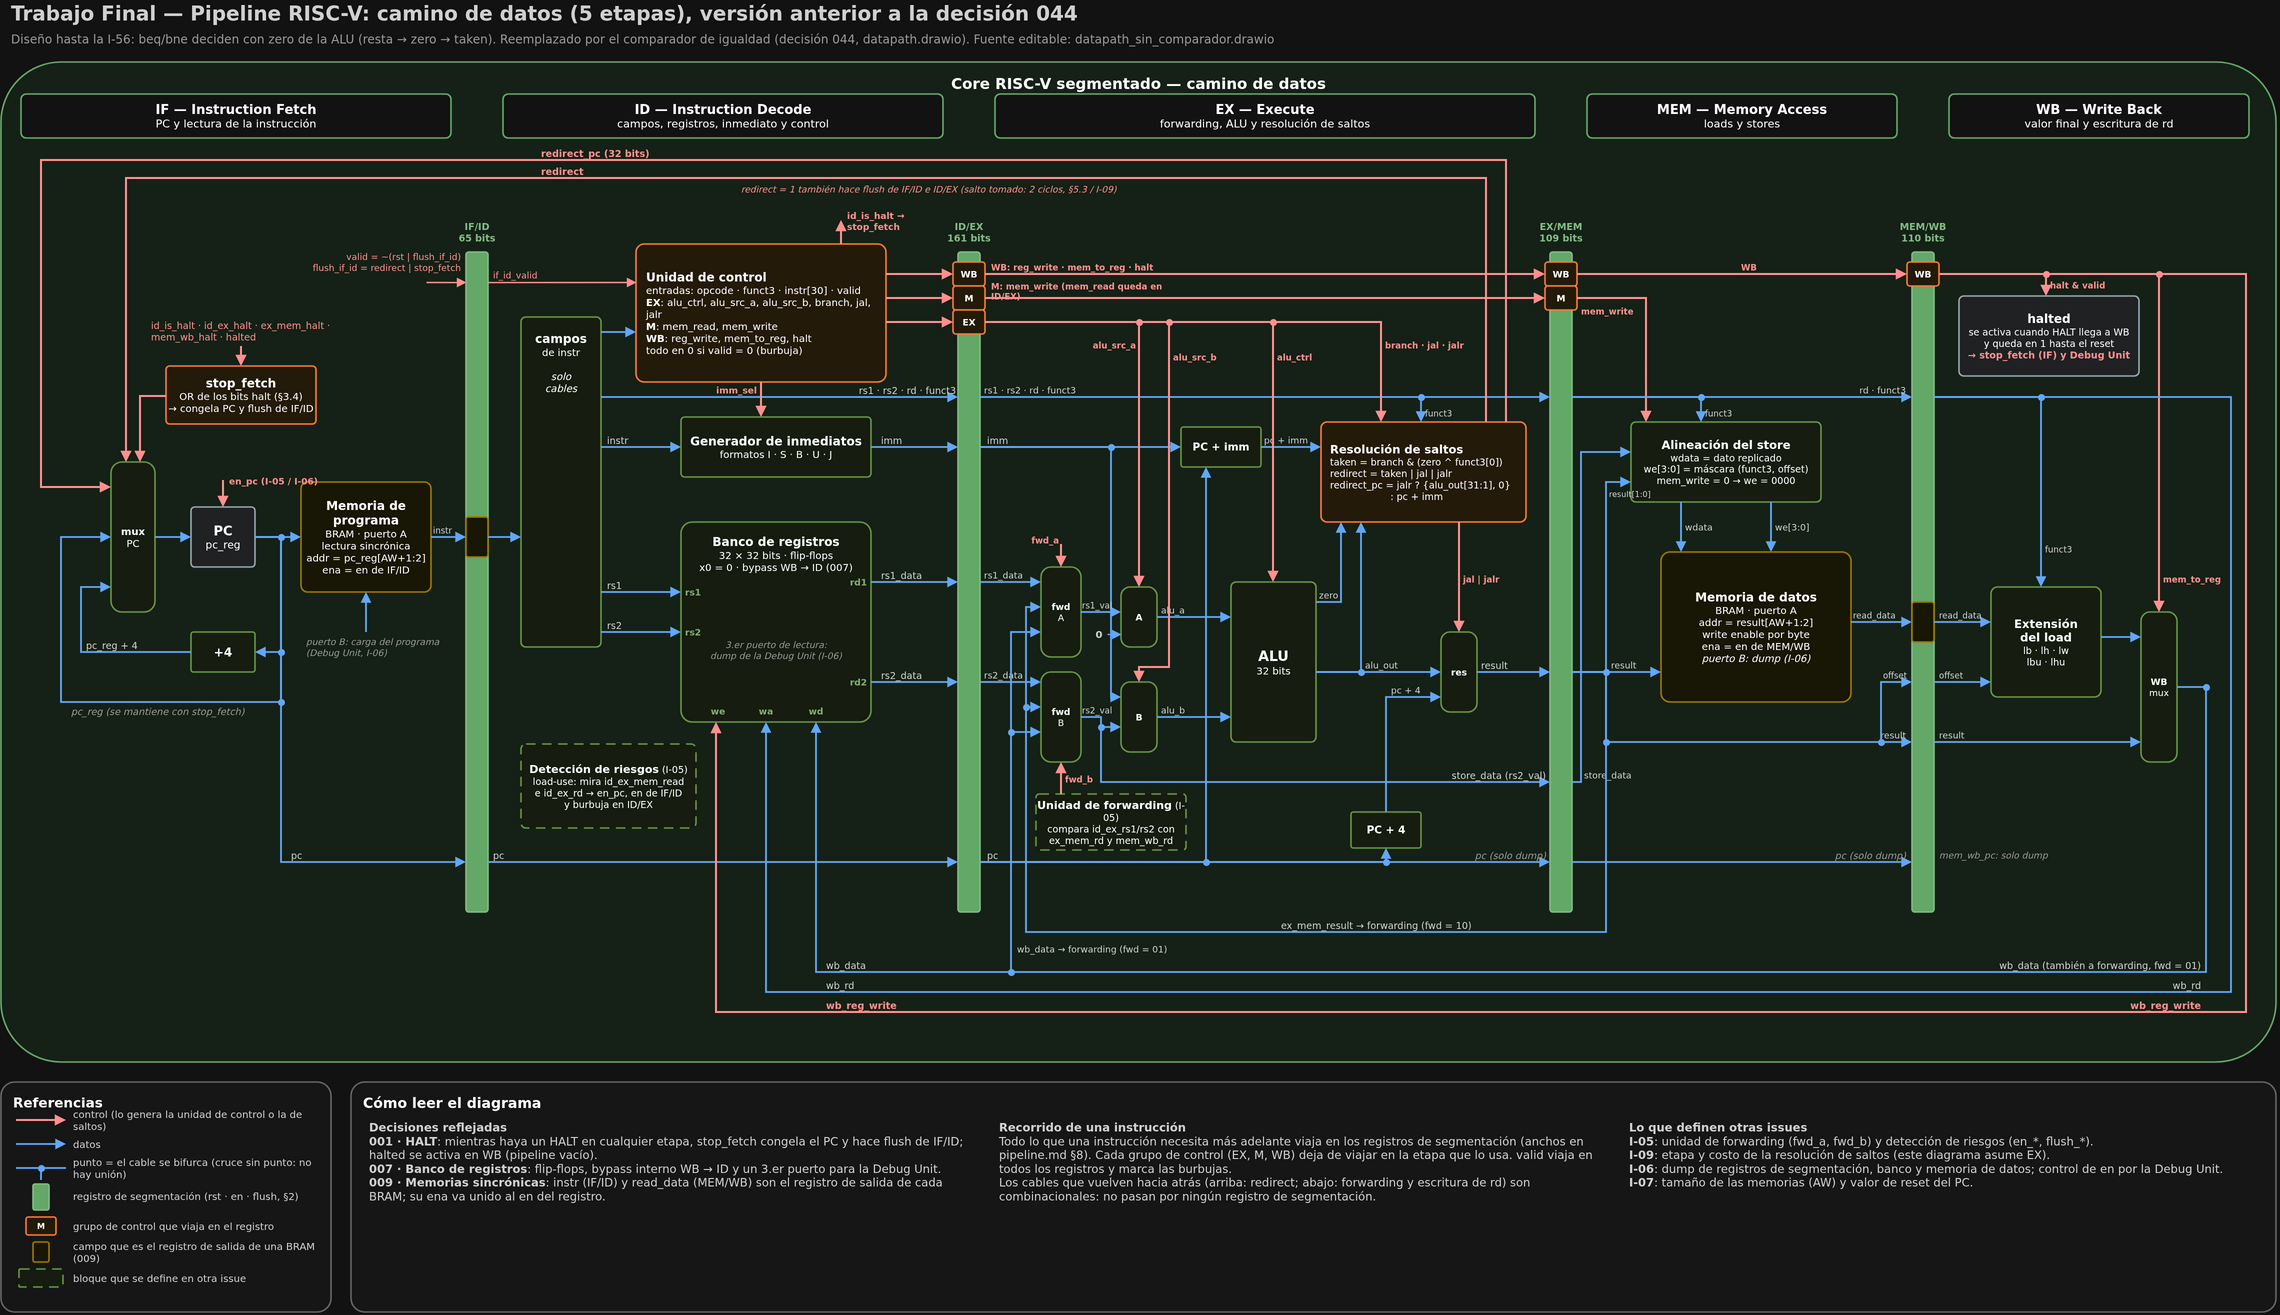
\includegraphics[width=\linewidth]{datapath_sin_comparador.png}
    \caption{Base: el salto decide con \texttt{zero} de la ALU.}
  \end{subfigure}\hfill
  \begin{subfigure}{0.49\linewidth}
    \centering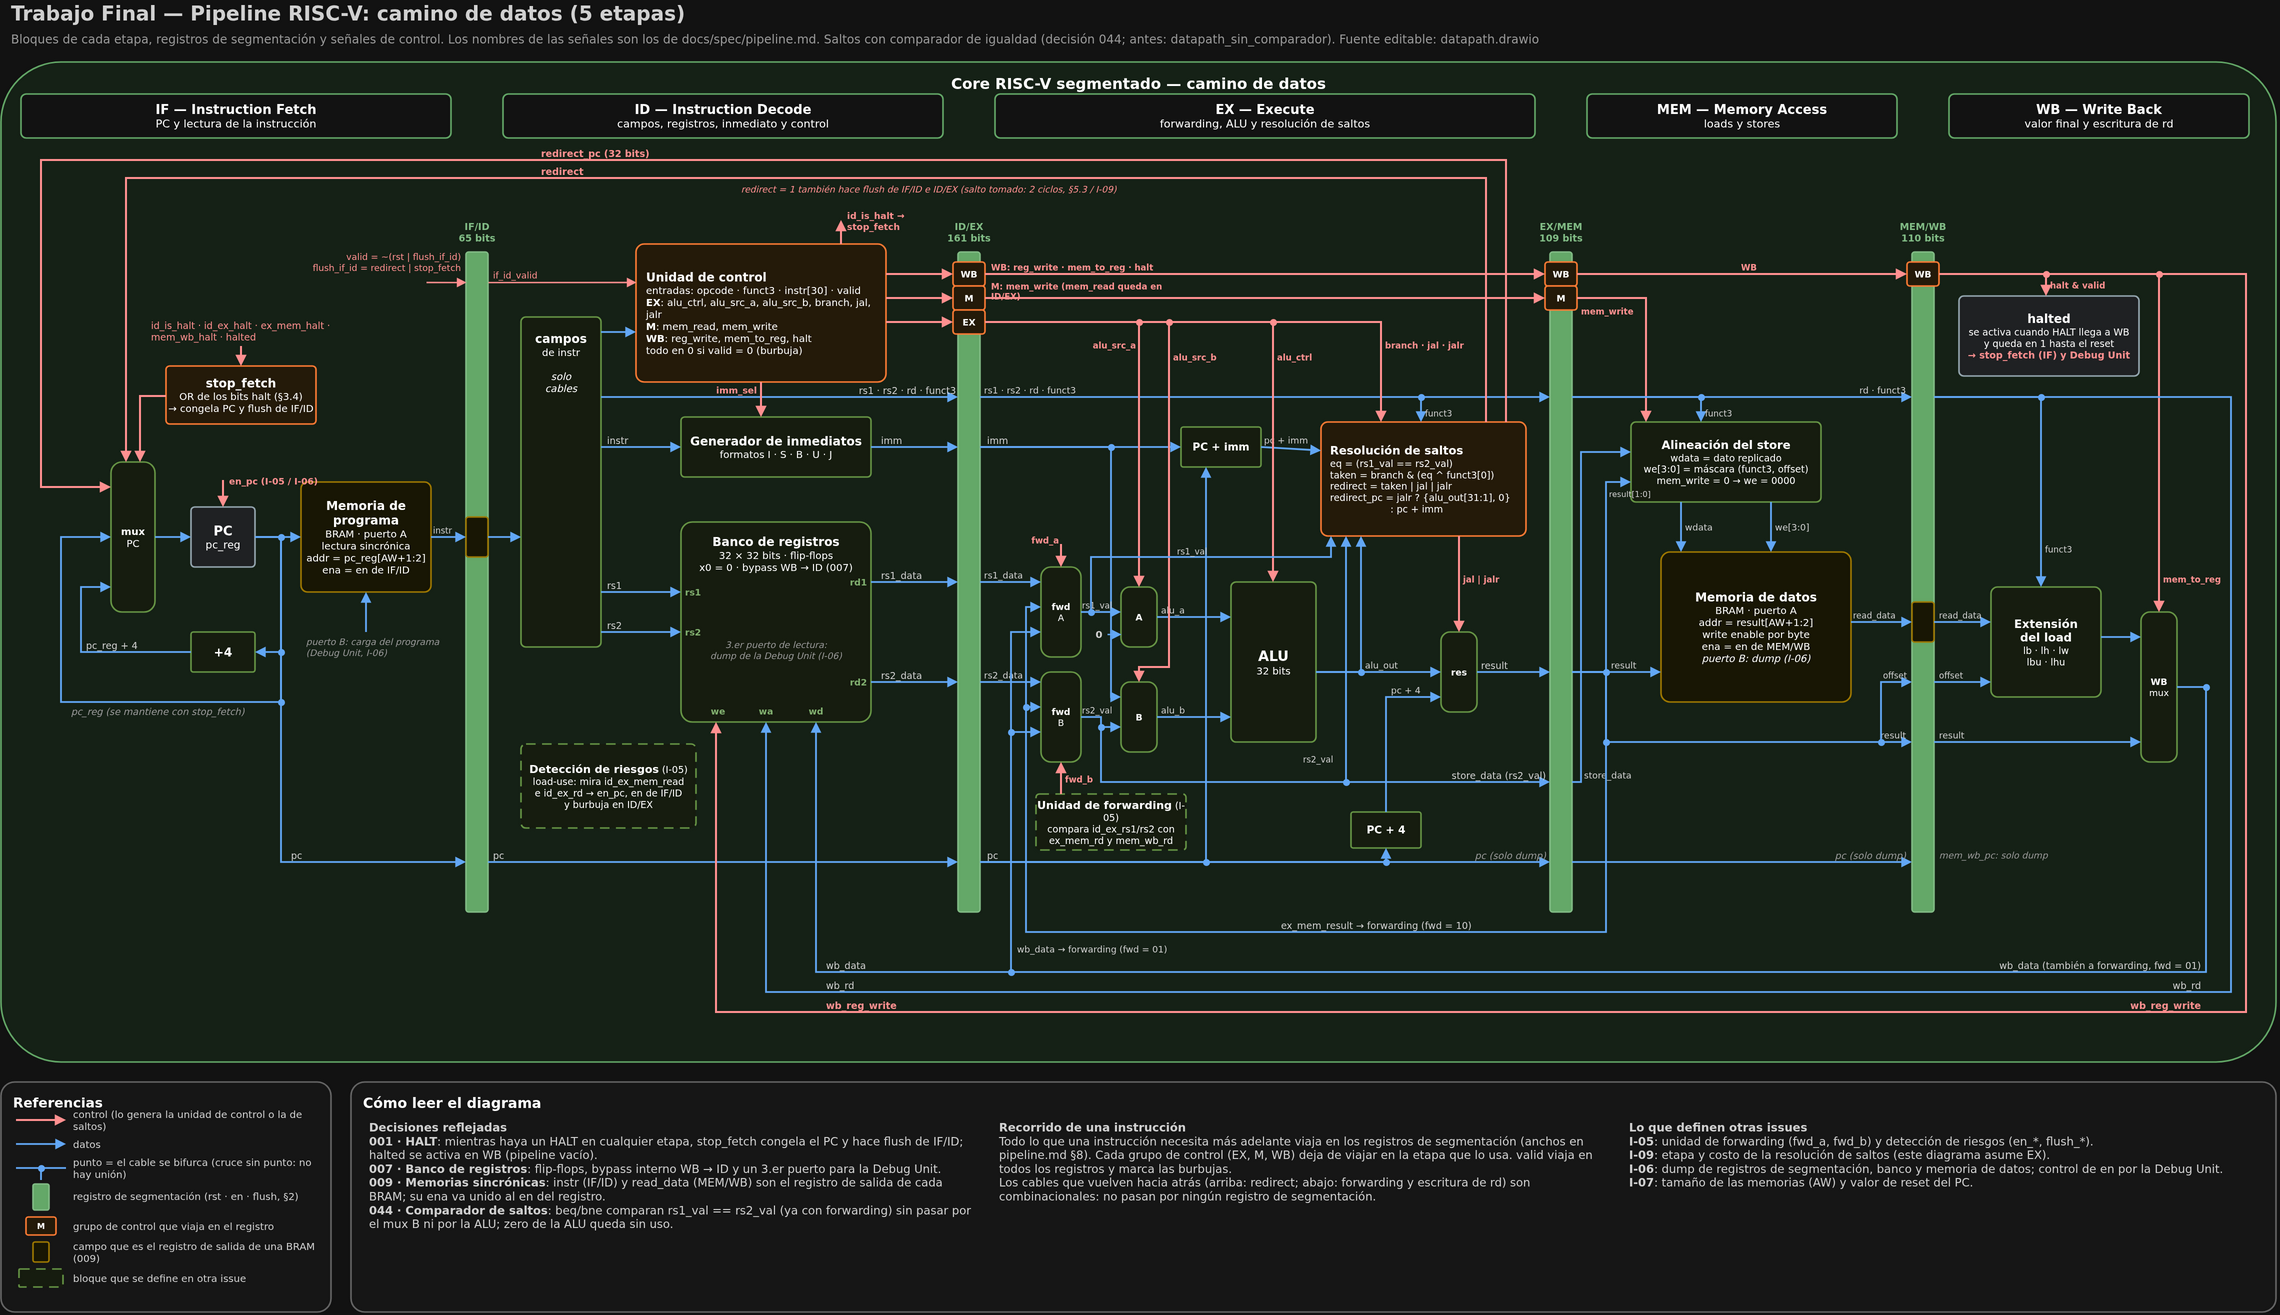
\includegraphics[width=\linewidth]{datapath.png}
    \caption{Final: comparador de igualdad (\decision{044}).}
  \end{subfigure}
  \caption{\textbf{Camino de datos antes y después del comparador.} El cambio está en EX: la
  decisión del salto deja de pasar por el mux del operando~B y la ALU.}
  \label{fig:comparador}
\end{figure}

\subsection{Barrido de frecuencias}

\begin{center}
\small
\begin{tabular}{@{}r r r r r r@{}}
  \toprule
  \textbf{MHz} & \textbf{WNS (ns)} & \textbf{TNS (ns)} & \textbf{Fallan} & \textbf{WHS (ns)} & \textbf{Peor camino (ns)} \\
  \midrule
  65  & $+1{,}418$ & 0 & 0 & $+0{,}066$ & 13,151 \\
  70  & $+1{,}111$ & 0 & 0 & $+0{,}037$ & 12,991 \\
  74  & $+1{,}078$ & 0 & 0 & $+0{,}037$ & 11,498 \\
  76  & $+0{,}229$ & 0 & 0 & $+0{,}045$ & 12,438 \\
  80  & $+0{,}412$ & 0 & 0 & $+0{,}046$ & 11,711 \\
  86  & $+0{,}409$ & 0 & 0 & $+0{,}051$ & 11,031 \\
  90  & $+0{,}288$ & 0 & 0 & $+0{,}098$ & 10,650 \\
  \textbf{92} & $\mathbf{+0{,}026}$ & 0 & 0 & $+0{,}037$ & 10,117 \\
  95  & $-0{,}449$ & $-5{,}893$ & 42 & $+0{,}037$ & 10,720 \\
  100 & $-0{,}714$ & $-30{,}251$ & 122 & $+0{,}075$ & 10,598 \\
  \bottomrule
\end{tabular}
\end{center}

La tabla es un extracto de las 16 frecuencias (\repo{docs/timing/i57_barrido/barrido.csv}). Muestra
tres cosas:

\begin{itemize}[nosep]
  \item \textbf{La cota de la medición a \qty{65}{\mega\hertz} era pesimista.} Suponía el mismo
        ruteo con otro reloj ($\approx$\qty{71,6}{\mega\hertz}). Con un reloj más exigente, la
        colocación y el ruteo guiados por timing acortan el camino: el retardo de datos baja de
        13,15 a 10,12~ns.
  \item \textbf{El resultado no es monótono.} De 76 a \qty{90}{\mega\hertz} el WNS sube y baja,
        y en algunas frecuencias el Clock Wizard elige otros divisores con menos jitter.
  \item \textbf{El flujo es determinista.} \qty{92}{\mega\hertz} se implementó tres veces (barrido,
        \repo{timing.tcl} y la GUI) con el mismo $+0{,}026$~ns.
\end{itemize}

Se eligió \textbf{\qty{92}{\mega\hertz}}, la máxima que cierra: el análisis estático ya usa el peor
caso de proceso, tensión y temperatura, así que con WNS $\geq 0$ el diseño funciona en la placa
(\decision{045}). El MMCM da exactamente $100 \times 48{,}875 / (5 \times 10{,}625) =
92{,}000$~MHz.

\subsection{Diseño final a \qty{92}{\mega\hertz}}

\begin{center}
\small
\begin{tabular}{@{}p{3.6cm} p{12cm}@{}}
  \toprule
  Período                 & 10,870~ns \\
  WNS / TNS (setup)       & $+0{,}026$~ns / 0, 0 de 5360 endpoints fallan \\
  WHS / THS (hold)        & $+0{,}037$~ns / 0 \\
  Peor camino             & \texttt{dmem\_bram} $\to$ WB $\to$ forwarding $\to$ comparador $\to$ \texttt{redirect} $\to$ flush de ID/EX; 10,117~ns, 9 niveles \\
  LUT / LUTRAM / FF       & 2907 (14\,\%) / 22 / 1884 (5\,\%) \\
  BRAM / MMCM / IO        & 2 RAMB36 (4\,\%) / 1 / 20 \\
  Consumo estimado        & 0,200~W (0,128 dinámico, de los que el MMCM es 0,120) \\
  UART                    & $\mathrm{DVSR} = 50$, 115\,000 baudios (\qty{-0,17}{\percent}) \\
  \bottomrule
\end{tabular}
\end{center}

A \qty{92}{\mega\hertz} varias etapas quedan en el límite, y todas empiezan en el
\emph{clock-to-out} de la BRAM de datos: EX/MEM a $+0{,}114$~ns (forwarding $\to$ ALU),
\texttt{pc\_reg} a $+0{,}171$~ns, el \emph{enable} de la memoria de programa a $+0{,}428$~ns. No hay
un único camino que, acortado, permita subir mucho más; por eso a \qty{95}{\mega\hertz} fallan 42
endpoints con destinos distintos.

\begin{figure}[H]
  \centering
  \begin{subfigure}{0.49\linewidth}
    \centering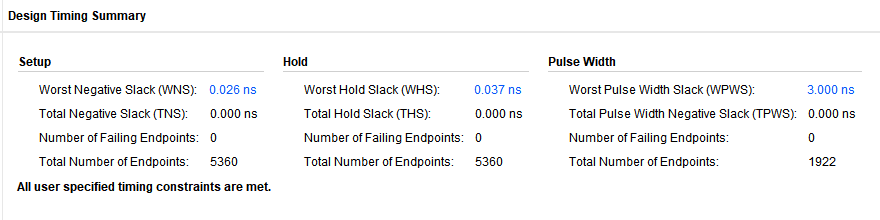
\includegraphics[width=\linewidth]{i57_92mhz/vivado_timing.png}
    \caption{\emph{Design Timing Summary} post-implementación.}
  \end{subfigure}\hfill
  \begin{subfigure}{0.49\linewidth}
    \centering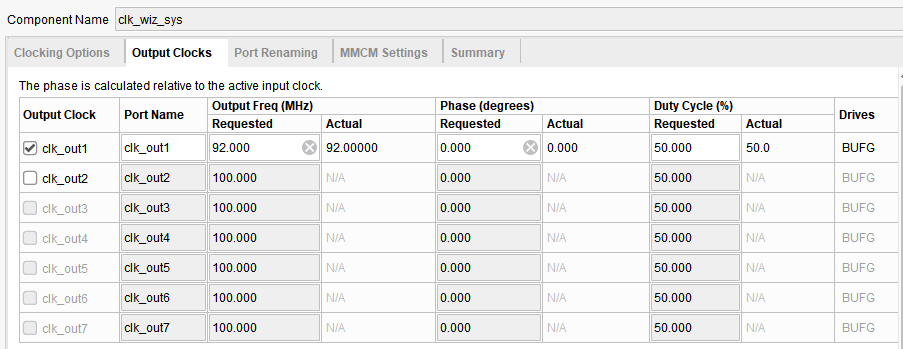
\includegraphics[width=\linewidth]{i57_92mhz/vivado_clk_wiz_salidas.png}
    \caption{Clocking Wizard: \qty{92,000}{\mega\hertz}.}
  \end{subfigure}
  \caption{\textbf{Implementación a \qty{92}{\mega\hertz} en Vivado.} Más capturas (MMCM, relojes,
  utilización, consumo y DRC) en \repo{docs/timing/i57_92mhz/}.}
  \label{fig:vivado92}
\end{figure}

\paragraph{Lo que no se aplicó.} El registro de salida de las BRAM sacaría su
\emph{clock-to-out} del camino crítico, y registrar \texttt{redirect} cortaría el camino del salto.
Las dos opciones suman ciclos (un load-use pasaría a costar 2 stalls y un salto tomado 3 ciclos) y
cambian el modelo y todos los \texttt{.exp}, a cambio de una frecuencia mayor. No se aplicaron: la
consigna evalúa la frecuencia y el análisis del camino, y con el comparador el diseño ya cumple
con margen positivo.

\subsection{Skew}
\label{sec:skew}

El diseño tiene un solo reloj (\texttt{clk\_out1\_clk\_wiz\_sys}) que sale del MMCM por un BUFG
hacia todos los elementos sincrónicos; el otro BUFG es la realimentación del MMCM. No hay
\texttt{BUFGCE}, divisores ni relojes generados con lógica.

\begin{center}
\small
\begin{tabular}{@{}p{5.4cm} p{10.2cm}@{}}
  \toprule
  \multicolumn{2}{@{}l}{\textbf{A \qty{92}{\mega\hertz}}} \\
  \midrule
  Skew del camino crítico de setup & $-0{,}073$~ns (0,7\,\% del período) \\
  Incertidumbre del reloj (jitter) & 0,129~ns \\
  Peores de setup por etapa        & de $-0{,}116$ a $+0{,}029$~ns \\
  Peores de hold por etapa         & de 0 a $+0{,}265$~ns (el mayor, de MEM/WB al banco, con slack $+0{,}455$~ns) \\
  \bottomrule
\end{tabular}
\end{center}

\begin{itemize}[nosep]
  \item \textbf{Setup}: un skew negativo (el reloj llega antes al destino) le quita tiempo al
        dato. Son 73~ps de 10,87~ns: pesa más el jitter, y ninguno de los dos limita la
        frecuencia. La limita el camino de datos.
  \item \textbf{Hold}: el peligro es el skew positivo, porque el dato nuevo puede pisar al viejo
        antes de capturarse. Todos los caminos tienen slack positivo. El hold no depende de la
        frecuencia: un WHS negativo no se arreglaría bajando el reloj.
  \item \textbf{Por qué es chico}: el árbol global de la FPGA está balanceado y el MMCM compensa el
        retardo de inserción con su realimentación (por eso Vivado muestra retardos de reloj
        negativos). Un reloj gateado para el paso a paso saldría por ruteo común, con skew del orden
        de los nanosegundos y violaciones de hold que Vivado no puede corregir. Es la razón de la
        \decision{018}.
\end{itemize}

% ===========================================================================
\section{Respuestas a las preguntas de la consigna}
\label{sec:preguntas}

Las respuestas completas, con las pruebas que respaldan cada una, están en
\repo{docs/decisiones/preguntas_consigna.md} (I-59).

\subsection{¿Hay que vaciar la memoria, los registros, el pipeline y la memoria de programa al
cargar un programa nuevo?}

Hay que vaciar la memoria de datos, los registros y el pipeline; la memoria de programa se
sobrescribe. Todo lo hace un solo comando, \texttt{LOAD} (decisiones 004 y 038):

\begin{center}
\small
\begin{tabular}{@{}l p{5.2cm} p{6.2cm}@{}}
  \toprule
  & \textbf{Qué hace \texttt{LOAD}} & \textbf{Por qué hace falta} \\
  \midrule
  Memoria de datos    & La pone en cero, junto con el mapa de palabras usadas & Si no, el programa nuevo lee datos del anterior y la memoria usada mezcla los dos \\
  Registros           & En cero, con el reset del core & El mismo programa daría resultados distintos según qué se corrió antes \\
  Pipeline            & Vacío, con el reset del core (todos los \texttt{valid} en 0) & Las instrucciones viejas en vuelo escribirían memoria o registros del programa nuevo \\
  Memoria de programa & Escribe el programa y rellena el resto con HALT & Vaciarla a cero no alcanza (\texttt{0x00000000} se ejecuta como NOP y el PC seguiría de largo); lo que importa es no ejecutar la cola de un programa anterior más largo \\
  \bottomrule
\end{tabular}
\end{center}

Lo prueban \repo{debug_load_tb.v} (reprogramar en los cuatro estados, también con el core corriendo
un lazo infinito) y la placa: \repo{placa.py} carga los 22 programas uno tras otro sin resetear la
placa, y todos dan su resultado esperado.

\subsection{¿Qué sucede si en la memoria no se encuentra una instrucción de parada?}

Al final de un programa no puede faltar, porque \texttt{LOAD} llena con HALT todo lo que el
programa no ocupa: un programa que ``se olvida'' el \texttt{halt} igual se detiene en la palabra
siguiente a la última. Quedan dos casos en que el procesador no se detiene solo:

\begin{itemize}[nosep]
  \item \textbf{Un lazo infinito}: el HALT nunca llega a ID y el core corre para siempre. Para eso
        está \texttt{STOP}, que baja \texttt{enable} y deja el core en \texttt{PAUSED} para
        inspeccionarlo; también sirven \texttt{RESET}, \texttt{LOAD} y el botón de reset.
  \item \textbf{Un programa de exactamente 1024 palabras sin HALT}: el PC llega a \texttt{0x1000},
        vuelve a la palabra 0 por el alias de direcciones y el programa se repite; el core levanta
        \texttt{imem\_fault}. Se corta igual con \texttt{STOP}.
\end{itemize}

En ningún caso se ejecuta basura de un programa anterior ni memoria sin inicializar.

\subsection{¿Cuál es el camino crítico del sistema?}

A \qty{92}{\mega\hertz}, post-implementación (sección~\ref{sec:timing}):

\begin{lstlisting}[style=verilog,numbers=none]
dmem_bram (clock-to-out, un load en MEM)
  -> mux de WB -> forwarding desde MEM/WB (operando del salto en EX)
  -> comparador de igualdad rs1_val == rs2_val
  -> taken -> redirect -> flush de ID/EX
slack +0,026 ns, 10,117 ns de datos, 9 niveles de logica
\end{lstlisting}

Es el caso de un \texttt{beq}/\texttt{bne} que compara un registro recién cargado. No es un camino
único: varias etapas quedan en el límite y todas salen de la BRAM de datos.

\subsection{¿Este camino crítico genera skew? ¿Qué consecuencias tiene?}

Muy poco: $-73$~ps en el camino crítico, el 0,7\,\% del período y menos que el jitter del MMCM
(129~ps). No limita la frecuencia ni rompe el hold, porque hay un solo reloj por un BUFG y el paso a
paso se hace con \texttt{enable} sin tocar el reloj (sección~\ref{sec:skew}).

\subsection{De encontrarse skew: frecuencia óptima, métricas y aplicarla}

El skew resultó despreciable, pero igual se buscó la frecuencia óptima, porque lo que la limita es
el camino crítico. \repo{scripts/barrido.tcl} implementó el diseño en 16 frecuencias de 65 a
\qty{100}{\mega\hertz}; la óptima es \textbf{\qty{92}{\mega\hertz}}, la máxima que cierra. Las
métricas salen de \repo{scripts/timing.tcl} (\texttt{report\_timing\_summary},
\texttt{report\_utilization}, \texttt{report\_power}, \texttt{report\_clock\_utilization}) y la
frecuencia se aplicó en el Clock Wizard y en el parámetro \texttt{CLK\_FREQ\_HZ} del top, del que
salen el divisor de la UART y el timeout de la Debug Unit. La regresión y la placa pasan completas a
\qty{92}{\mega\hertz}, e \texttt{INFO} informa \texttt{clk\_khz = 92000}.

% ===========================================================================
\section{Uso del sistema}
\label{sec:uso}

\subsection{Requisitos}

\begin{itemize}[nosep]
  \item Vivado~2024.2 y una Basys~3.
  \item Python~3.11 o más nuevo, con \texttt{pyserial} y \texttt{textual}
        (\repo{tools/debugger/requirements.txt}). El ensamblador y el modelo de referencia no tienen
        dependencias.
\end{itemize}

\subsection{Generar el bitstream y programar la placa}

El proyecto de Vivado no se versiona: se regenera desde las fuentes.

\begin{enumerate}[nosep]
  \item En Vivado, \emph{Tools $>$ Run Tcl Script} con \repo{scripts/create_project.tcl}. Crea el
        proyecto \texttt{riscv\_basys3} en \repo{build/}, con los IP del Clock Wizard y de las BRAM.
  \item \emph{Generate Bitstream} y, con la placa conectada, \emph{Open Hardware Manager $>$
        Program Device}.
  \item Después de programar, LD0 (\texttt{NO\_PROG}) queda encendido y LD15 late a
        \qty{2}{\hertz}.
\end{enumerate}

\subsection{Usar el debugger}

\begin{lstlisting}[language=bash,numbers=none]
pip install -r tools/debugger/requirements.txt
python tools/debugger/debugger.py --port COM8 --prog sw/demo/demo_datos.s
\end{lstlisting}

El puerto es el de número más alto de los dos que crea el FT2232 de la placa (en Linux,
\texttt{/dev/ttyUSB1}). Con \texttt{F1} se conecta, \texttt{F2} carga el programa, \texttt{F10}
avanza un ciclo y \texttt{F5} ejecuta hasta el HALT (tabla de teclas en la
sección~\ref{sec:interfaz}).

\subsection{Otros comandos}

\begin{center}
\footnotesize
\begin{tabular}{@{}l p{5.6cm}@{}}
  \toprule
  \textbf{Comando} & \textbf{Para qué} \\
  \midrule
  \texttt{python tools/assembler/asm.py prog.s -o prog.lst}        & Ensamblar y ver el listado con direcciones \\
  \texttt{python tools/isasim/sim.py prog.s --exp auto}            & Correr el modelo y compararlo con el \texttt{.exp} \\
  \texttt{python tools/debugger/comparar.py COM8 prog.s --cada-ciclo} & Comparar la placa con el modelo en cada ciclo \\
  \texttt{python tools/debugger/placa.py COM8}                     & Prueba en placa de los 22 programas del plan \\
  \texttt{python scripts/regresion.py} + \texttt{regresion.tcl}    & Regresión completa en xsim \\
  \texttt{python -m pytest sw tools/assembler tools/isasim}        & Tests de las herramientas \\
  \bottomrule
\end{tabular}
\end{center}

\subsection{Programas de demostración}
\label{sec:demo}

Dos programas cortos en \repo{sw/demo/} (I-58) muestran entre los dos todos los mecanismos de
riesgo, recorridos en paso a paso con el debugger:

\begin{center}
\small
\begin{tabular}{@{}l r r p{8cm}@{}}
  \toprule
  \textbf{Programa} & \textbf{Instr.} & \textbf{Ciclos} & \textbf{Qué muestra} \\
  \midrule
  \repo{demo_datos}   & 10 & 15 & Forwarding hacia la ALU y hacia el dato del store, bypass del banco, carga-uso y load sin dependencia \\
  \repo{demo_control} & 15 & 44 & Lazo con \texttt{bne} hacia atrás, forwarding al comparador, \texttt{lw} seguido de \texttt{beq}, flush y un HALT en el camino equivocado \\
  \bottomrule
\end{tabular}
\end{center}

\begin{figure}[H]
  \centering
  \begin{subfigure}{0.49\linewidth}
    \centering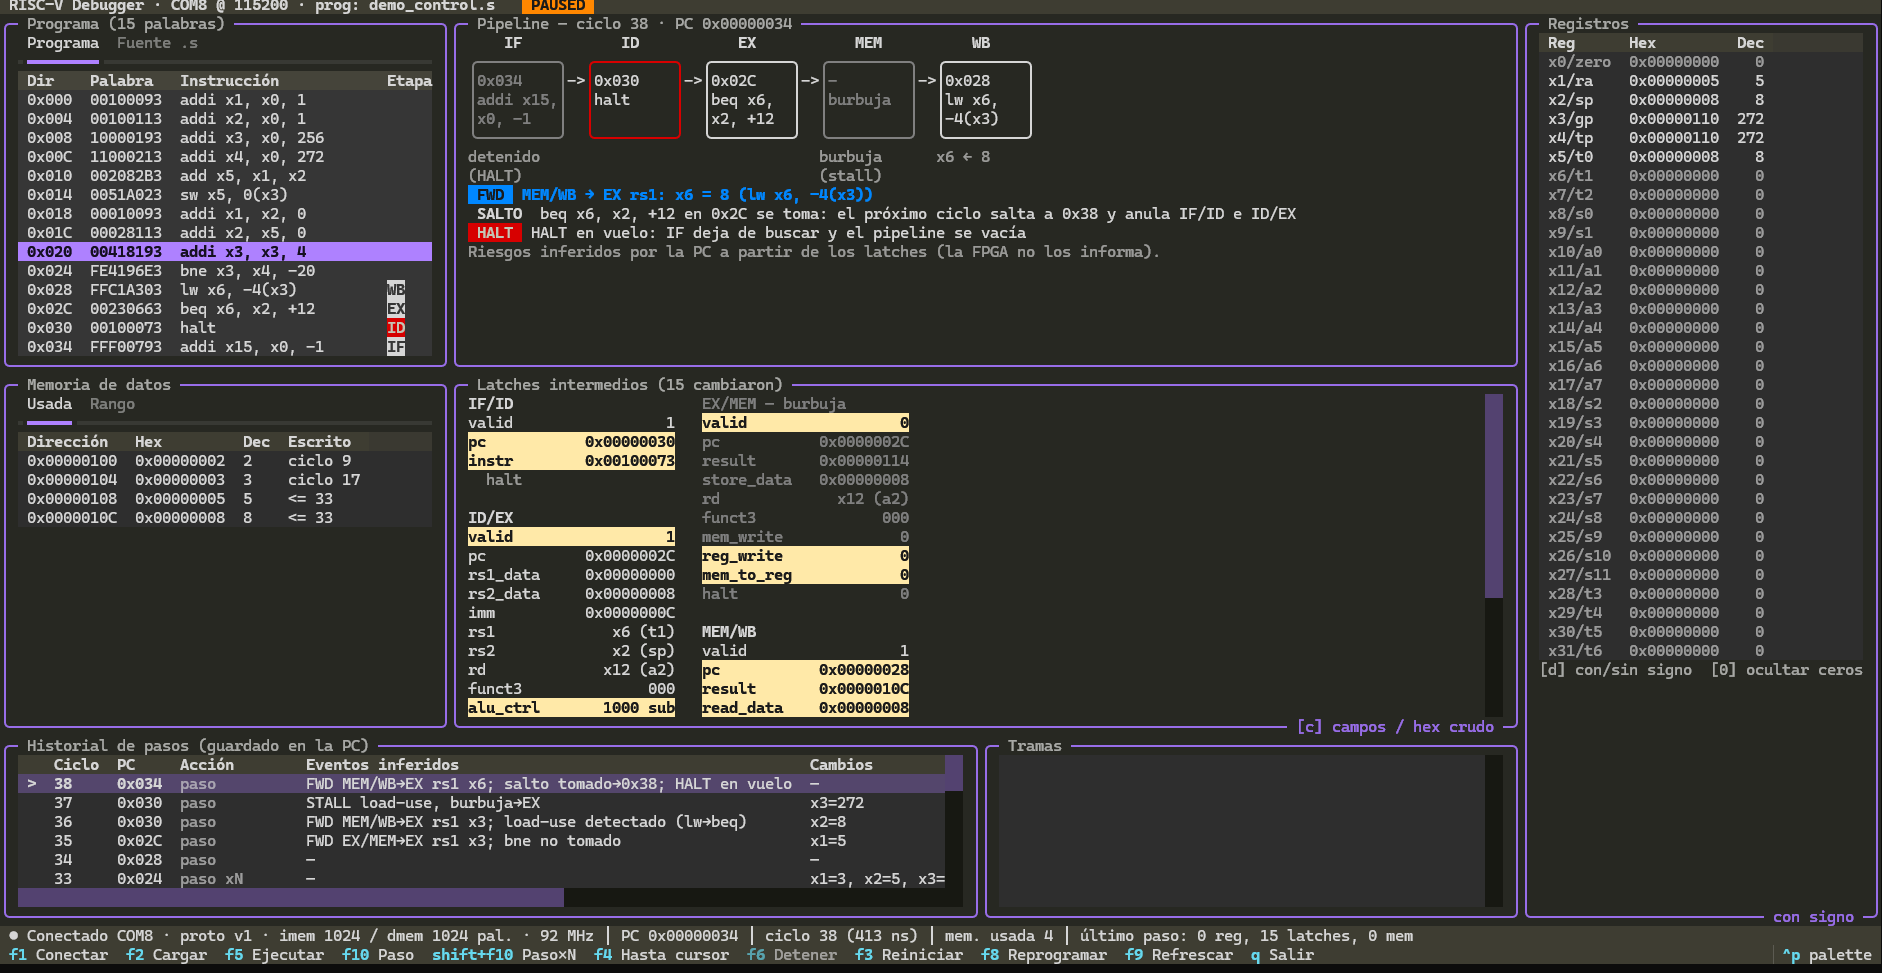
\includegraphics[width=\linewidth]{debugger_demo_control_ciclo38.png}
    \caption{Ciclo 38: el \texttt{beq} recibe \texttt{x6} desde MEM/WB y se toma; el HALT del
    camino equivocado está en ID.}
  \end{subfigure}\hfill
  \begin{subfigure}{0.49\linewidth}
    \centering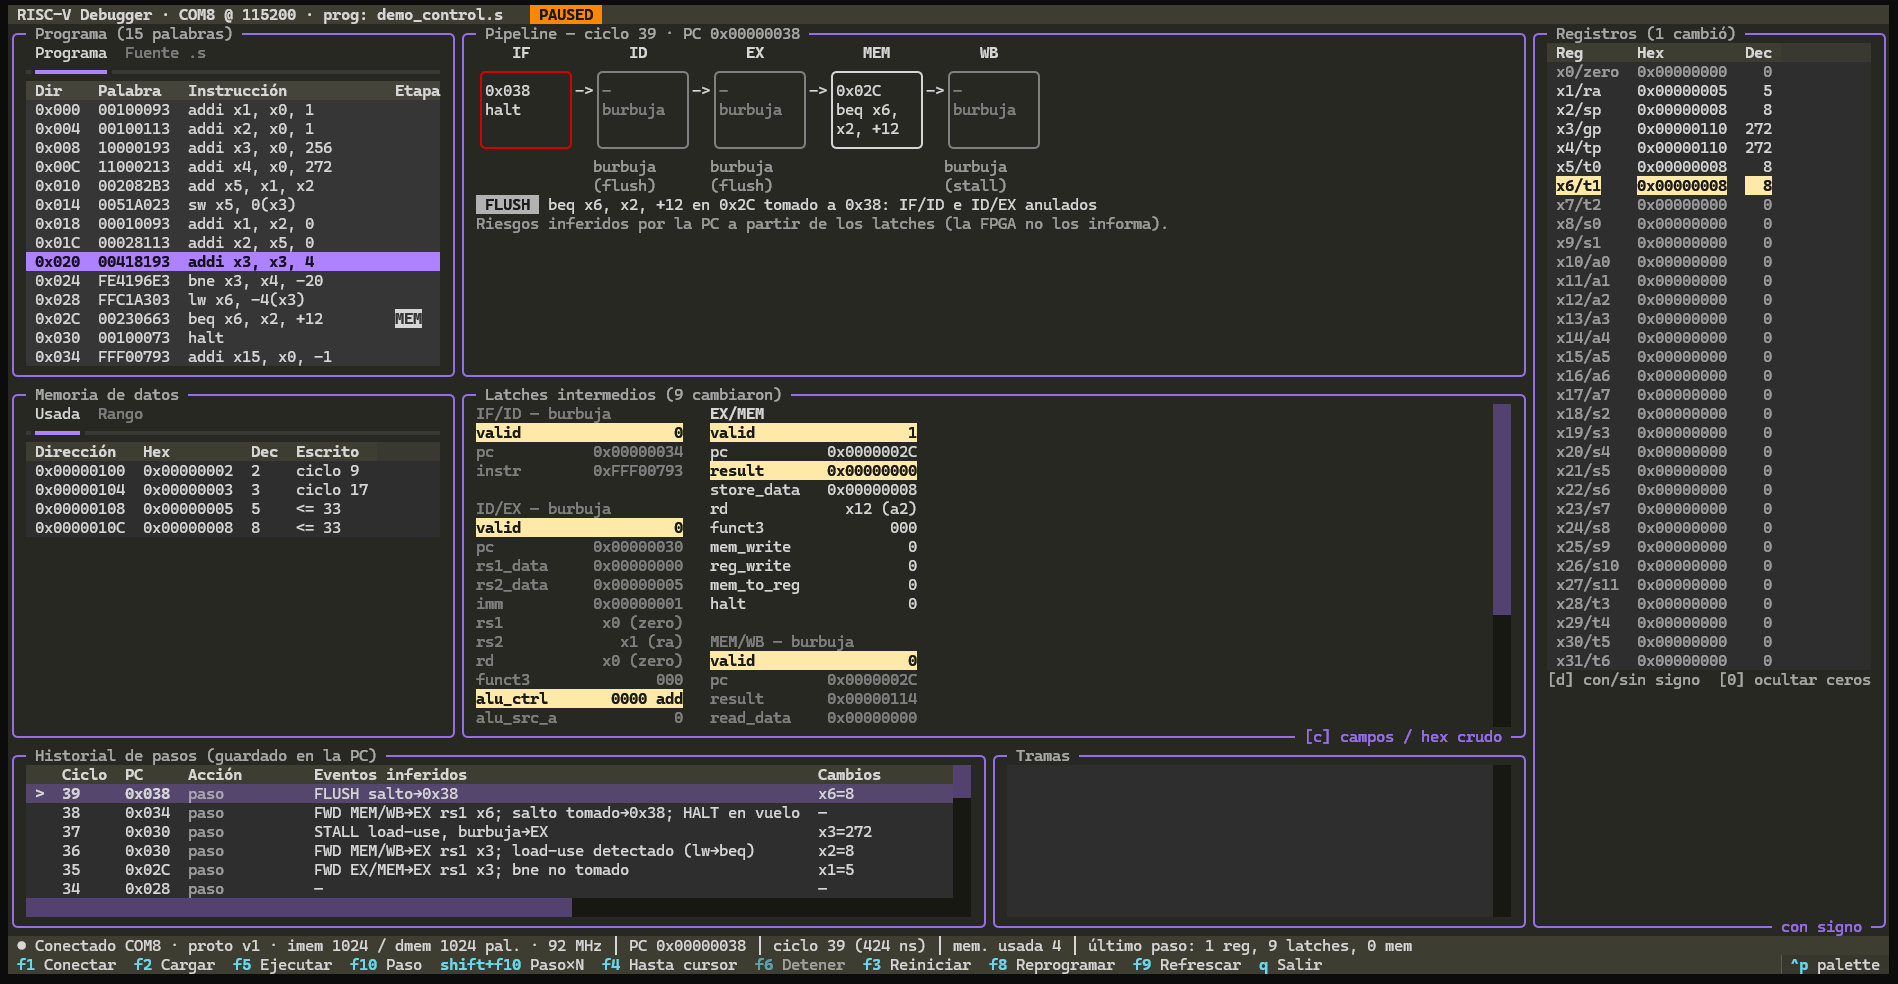
\includegraphics[width=\linewidth]{debugger_demo_control_ciclo39.png}
    \caption{Ciclo 39: flush de IF/ID e ID/EX; el HALT se anula y el core sigue en
    \texttt{PAUSED}.}
  \end{subfigure}
  \caption{\textbf{\repo{demo_control} en la placa.} El HALT en el camino equivocado no detiene el
  procesador.}
  \label{fig:demo_control}
\end{figure}

El guion de la demostración y la cobertura ciclo por ciclo están en \repo{sw/demo/README.md}.

% ===========================================================================
\section{Conclusiones}
\label{sec:conclusiones}

Se implementó y verificó en la Basys~3 un procesador RISC-V RV32I segmentado en cinco etapas, con
forwarding, detección de carga-uso y flush por saltos, controlado desde la PC por una Debug Unit que
carga programas, ejecuta de corrido o de a un ciclo y vuelca registros, latches y memoria de datos
usada. Funciona a \qty{92}{\mega\hertz}, la máxima frecuencia que cumple timing, con un solo reloj y
sin intervenirlo.

\paragraph{Lo que funcionó.}
\begin{itemize}[nosep]
  \item \textbf{Especificar antes de codificar.} Las interfaces de cada módulo y el contrato de
        nombres de los registros de segmentación se fijaron en \repo{docs/spec/} antes del RTL. El
        mismo empaquetado de los latches sirve para la traza del modelo, el banco de pruebas y el
        volcado de la Debug Unit, así que la placa se compara con el modelo sin traducciones.
  \item \textbf{Integrar etapa por etapa.} Cada error quedó acotado a la última etapa agregada.
  \item \textbf{Dos oráculos independientes y mutantes.} Con los \texttt{.exp} a mano y el
        modelo escritos por separado, cada diferencia señalaba qué revisar (la ISA, el modelo o el
        RTL); los mutantes mostraron qué programas faltaban para cubrir cada mecanismo.
  \item \textbf{Medir antes de optimizar.} La hipótesis del camino crítico de la \decision{012} se
        confirmó en el qué y se corrigió en el cómo (el desplazador, no la resta), y eso llevó a una
        mejora que no cambió ciclos ni resultados: el comparador de igualdad.
\end{itemize}

\paragraph{Limitaciones y trabajo futuro.}
\begin{itemize}[nosep]
  \item Sin excepciones: los accesos inválidos se truncan y dejan un aviso (\decision{015}).
  \item Los saltos tomados cuestan 2 ciclos. Una predicción de saltos hacia atrás o el forwarding
        hacia MEM para un \texttt{sw} después de un \texttt{lw} ahorrarían ciclos a cambio de más
        lógica en el camino crítico.
  \item A \qty{92}{\mega\hertz} varias etapas quedan en el límite y todas empiezan en la BRAM de
        datos; subir más exige registrar su salida o la redirección, con un ciclo más por load o por
        salto.
\end{itemize}


\appendix
% ===========================================================================
% Armado desde el título de cada nota de docs/decisiones/.
\section{Decisiones de diseño}
\label{anx:decisiones}

Cada nota de \repo{docs/decisiones/} tiene el contexto, las opciones consideradas, la decisión y
sus consecuencias. Una decisión no se edita para cambiarla: se escribe una nueva que la reemplaza.

\begin{longtable}{@{}r p{13.4cm}@{}}
  \toprule
  \textbf{N.\textdegree} & \textbf{Decisión} \\
  \midrule
  \endhead
  001 & Codificación y comportamiento de la instrucción HALT \\
  002 & Formato de trama del protocolo de debug \\
  003 & Baudrate de la UART: 115200 \\
  004 & LOAD como único mecanismo de carga y reprogramación \\
  005 & Cómo se determina la ``memoria de datos usada'' \\
  006 & Debug Unit con dos FSM independientes \\
  007 & Banco de registros: implementación y conflicto de lectura/escritura entre ID y WB \\
  008 & Interfaz de PC: TUI con Textual \\
  009 & Integración de las memorias de lectura sincrónica (BRAM) en el pipeline \\
  010 & Convenciones de código RTL \\
  011 & Detección de load-use conservadora y sin forwarding hacia MEM \\
  012 & Resolución de saltos en EX, sin predicción \\
  013 & Tamaño y mapa de direcciones de las memorias \\
  014 & Implementación de las memorias con BRAM y escritura de la memoria de programa por el puerto B \\
  015 & Accesos desalineados y fuera de rango: se truncan y dejan un aviso \\
  016 & Acceso por byte y media palabra con \emph{byte write enable} de la BRAM \\
  017 & Ensamblador propio, formatos de salida y validación \\
  018 & Ejecución paso a paso sin intervenir el clock \\
  019 & Programas de prueba: estado inicial, variantes con nop y convenciones de sw/ \\
  020 & Modelo de referencia: semántica de la ISA más pipeline ciclo a ciclo \\
  021 & Banco de pruebas incremental: carga, comparación y cortes por etapa \\
  022 & Memoria de programa: sin reset del registro de salida y contenido inicial sin archivo \\
  023 & Interfaz de debug del core y estructura de la etapa IF \\
  024 & Instrucciones no soportadas: decodificación solo por opcode \\
  025 & Filtro de palabras fuera de isa.md en el toolchain \\
  026 & Control de la ALU en ID, sin módulo aparte \\
  027 & Memoria de datos: qué lógica de MEM va en \texttt{dmem} \\
  028 & Regresión del pipeline por lotes en Vivado \\
  029 & Modo del modelo de referencia durante las integraciones de M8 \\
  030 & Corridas sin \texttt{+FINAL} en la regresión por lotes \\
  031 & Mutantes del RTL para la regresión \\
  032 & Testbenches unitarios en la regresión por lotes \\
  033 & Varias corridas en una simulación de \texttt{pipeline\_tb} \\
  034 & Desensamblador: \texttt{rvasm} envuelve el del modelo de referencia \\
  035 & UART de la Debug Unit: interfaz de bytes y FIFO de recepción \\
  036 & FSM de protocolo de la Debug Unit: alcance, puertos y reglas de validación \\
  037 & FSM de ejecución de la Debug Unit: STEP, enable, prioridades y gancho de la carga \\
  038 & Carga de programa en la Debug Unit: contrato con la FSM de ejecución y con el mapa de usadas \\
  039 & Volcado de estado de la Debug Unit: latches, mapa de usadas y fuente del payload \\
  040 & Interfaz de usuario: capas \texttt{model} y \texttt{session}, hilos y corte con la I-53 \\
  041 & Reset del sistema en la placa: botón sincronizado y reset de encendido \\
  042 & Reloj del sistema a 65 MHz con el Clock Wizard para la prueba en placa \\
  043 & Vista del pipeline: instrucción de cada etapa, riesgos inferidos, historial y F4 \\
  044 & Comparador de igualdad para decidir los saltos \\
  045 & Reloj del sistema a 92 MHz, la máxima frecuencia del barrido \\
  \bottomrule
\end{longtable}


\end{document}
